\documentclass[12pt,a4paper]{article}
\usepackage{composites2019}
\usepackage{booktabs}

\begin{document}
\thispagestyle{empty}

\vspace*{-3.4cm}
\begin{table}[!h]
\begin{tabular}{r}
\hspace*{5.5cm} \scriptsize \textsf{7th ECCOMAS Thematic Conference on the Mechanical Response of Composites} \\
\hspace*{5.5cm} \scriptsize \textsf{ COMPOSITES 2019} \\
\hspace*{5.5cm} \tiny \textsf{A. Turon, P. Maimí \& M. Fagerström (Editors)}
\end{tabular}
\end{table}

\begin{center}
\title{ESTIMATING THE AVERAGE SIZE OF FIBER/MATRIX INTERFACE CRACKS IN UD AND CROSS-PLY LAMINATES}
\end{center}
\begin{center}
\textbf{\underline{Luca Di Stasio}$^{1,2,*}$, Janis Varna$^{1}$, Zoubir Ayadi$^{2}$} \\ [7pt]
\small{$^1$~Lule\aa\ University of Technology, University Campus, SE-97187 Lule\aa, Sweden}  \\  [2pt]  
\small{$^2$~Universit\'e de Lorraine, EEIGM, IJL, 6 Rue Bastien Lepage, F-54010 Nancy, France}  \\  [2pt]
\small{$^*$~\texttt{luca.di.stasio@ltu.se}} \\
\end{center}


\paragraph{Keywords:} Fiber Reinforced Polymer (FRP), Debonding, Linear Elastic Fracture Mechanics (LEFM).

\paragraph{Summary:} \textit{Initiation and propagation of fiber/matrix interface cracks are analyzed in Representative Volume Elements (RVEs) of UD and cross-ply laminates. By studying the distribution of stresses at the fiber/matrix interface in the undamaged case, an estimate of the initial flaw size is derived. By adopting a 2-parameters energy-based criterion for propagation~\cite{Hutchinson1991}, we then proceed to the estimation of the expected average debond size in different microstructural arrangements. Finally, the results are compared with microscopic observations available in the literature~\cite{Correa2018}.}

\section{INTRODUCTION}

Characterization of initiation and growth of fiber/matrix interface cracks (or debonds) in Fiber Reinforced Polymer (FRP) composites has proven elusive, particularly the determination of initial flaw size and maximum debond extension. Different methodological approaches exist in the literature to study debond growth, namely Linear Elastic Fracture Mechanics (LEFM)~\cite{Paris2007}, Finite Fracture Mechanics (FFM)~\cite{Mantic2009}, Cohesive Zone Modeling (CSM)~\cite{Canal2012}, as well as several initiation physics-based criteria, such as tensile failure of the interface~\cite{Paris2007}, local cavitation-induced brittle matrix failure~\cite{Asp1996a,Asp1996b}, local matrix plasticization~\cite{Canal2012}, local nucleation plane~\cite{Carraro2014}. We propose here an attempt to evaluate initiation and propagation of debonds by taking into account the uncertainty in failure criteria and mechanisms evident from the literature. We thus aim to estimate a range of plausible values of initial flaw size and maximum debond size by: first, analyzing the stress distribution at the fiber/matrix interface in the absence of damage in Representative Volume Elements (RVEs) of UD and cross-ply laminates; second, determining the angular size of the regions where $\sigma\geq99\%\sigma_{max}$, $\sigma\geq95\%\sigma_{max}$ and $\sigma\geq90\%\sigma_{max}$ whith $\sigma_{max}$ the stress peak value, which provides an estimate of the expected initial flaw size; third, estimating the Mode I critical Energy Release Rate (ERR) of the interface crack, based on the values of initial flaw size and assuming a mixed-mode energy-based debond propagation criterion~\cite{Hutchinson1991}; fourth, comparing total ERR with the critical ERR provided by the propagation criterion~\cite{Hutchinson1991}. Finally, the estimated range of maximum debond size is compared with the results of microscopical observations of cross-ply specimens reported in~\cite{Correa2018}.

\section{RVE MODELS AND FE DISCRETIZATION}

In this contribution, we analyze debond initiation and propagation in Representative Volume Elements (RVEs) of Uni-Directional (UD) composites and $\left[0_{m\cdot k\cdot2L}^{\circ},90_{k\cdot2L}^{\circ},0_{m\cdot k\cdot2L}^{\circ}\right]$ laminates. Given a global reference frame with axis $x$, $y$ and $z$, both types of composites are modeled as plates lying in the $x-y$ plane, with the through-the-thickness direction thus aligned with the $z$ axis. The UD composite $0^{\circ}$ direction is parallel to the $y$ axis, while the cross-ply $0^{\circ}$ direction is parallel to the $x$ axis. Both composites are loaded in tension along the $x$ axis, which thus corresponds to: transverse loading of the UD specimen; axial loading of the cross-ply specimen. In both composites, damage is present only in the form of fiber/matrix interface cracks, or debonds. In cross-plies, debonds are assumed to be present only in the central ${90^{\circ}}$ ply. Given that: first, in the presence of a load in the $x$-direction, in both lay-ups the $y$-strain due to Poisson's effect is very small; second, debond size is assumed to be considerably larger in the fiber than in the arc direction~\cite{Zhang1997}; we can consider $2D$ models under plane strain conditions defined in the $x-z$ plane. Although generalized plane strain conditions would represent a more appropriate modeling choice, it would limit the ability to compare with previous results. Simple plane strain conditions are thus preferred. UD composites and $90^{\circ}$ plies are characterized by a regular microstructure following a square-packing configuration of fibers, built through the repetition of a one-fiber unit cell along the horizontal and the vertical direction. This unit cell is a square with the center occupied by one fiber of radius $R_{f}=1\ \mu m$ and the rest of the element constituted by matrix. The size of the one-fiber unit cell is $2L\times 2L$, such that:

\begin{equation}\label{eq:LVf}
L=\frac{R_{f}}{2}\sqrt{\frac{\pi}{V_{f}}},
\end{equation}

where $V_{f}$ is the fiber volume fraction, here assumed to be $60\%$. It is worth to specify at this point that the choice $R_{f}=1\ \mu m$ is arbitrary and stems from the fact that ERR, in the contest of a linear elastic solution as the one considered in this article, is proportional to the geometrical dimensions of the model. Simplicity is thus the main reason for this choice. Also, $V_{f}$ is always the same in the one-fiber unit cell and the entire RVE, i.e. no fiber clustering is analyzed in this work. In the case of cross-ply laminates, the $0^{\circ}$ layer is homogenized with properties evaluated according to the Concentric Cylinders Assembly with Self-Consistent Shear (CCA-SCS) model~\cite{Hashin1983,Christensen1979}. A glass fiber-epoxy system is considered for both UDs and cross-ply laminates. Material properties are reported in Table~\ref{tab:phaseprop}.

\begin{table}[!htbp]
 \centering
 \caption{Summary of mechanical properties of fiber, matrix and UD layer.}%$E$ stands for Young's modulus, $\mu$ for shear modulus and $\nu$ for Poisson's ratio. Indexes $L$ and $T$ stand respectively for \emph{longitudinal} and \emph{transverse}.}
 \begin{tabular}{ccccccc}
\textbf{Material} & \textbf{$V_{f}\left[\%\right]$}\  & \textbf{$E_{L}\left[GPa\right]$}\ & \textbf{$E_{T}\left[GPa\right]$}\  & \textbf{$G_{LT}\left[GPa\right]$} &\textbf{$\nu_{LT}\left[-\right]$} & \textbf{$\nu_{TT}\left[-\right]$} \\
\midrule
Glass fiber &-   & 70.0 & 70.0  & 29.2 & 0.2  & 0.2\\
Epoxy    &-& 3.5 & 3.5   & 1.25 &  0.4& 0.4\\
UD&60.0&43.442&13.714& 4.315& 0.273&0.465\\
\end{tabular}
\label{tab:phaseprop}
\end{table}

The use of coupling conditions allows the study of a Repeating Unit Cells (RUC) of reduced size with respect to the corresponding RVE, which translates in a gain in terms of computational time and memory usage during the evaluation of Finite Element (FE) solution. The RVEs studied in this article are reported in Figure~\ref{fig:rves} with the corresponding RUC highlighted by dashed line (in blue in the online color version) and with symmetry and coupling conditions represented by rollers (
\includegraphics[scale=0.5]{roller.pdf}). Details about the central one-fiber unit cell are shown in Figure~\ref{fig:ruc}. Notice that the analysis, in terms of stresses and Energy Release Rate (ERR), is conducted on this central one-fiber unit cell, both in the case of an undamaged and of a partially debonded fiber.\\
Nomenclature and main features of the RVEs studied are described in the following.

\begin{description}
\item [$\mathbf{n\times k-free}$, Figure~\ref{fig:rves-a}: ]UD composite with thickness $t_{UD}=k\cdot2L$, where $k$ is the number of fiber ``rows'' in the vertical (through-the-thickness) direction and $2L$ the side length of the one-fiber unit cell as defined in Equation~\ref{eq:LVf}. Debonds appear only in the central fiber ``row'' with $n-1$ fully bonded fibers in between, where $n$ is the number of fibers present in the RUC along the horizontal direction.
\item [$\mathbf{n\times k-coupling}$, Figure~\ref{fig:rves-b}: ]UD composite with infinite thickness. Debonds appear every $k-1$ fully bonded fibers along the vertical direction in a fiber ``column'', fiber ``columns'' containing debonds appear every $n-1$ ``columns'' of fully bonded fibers. Debonds are placed on the same side of the partially debonded fiber inside the same fiber ``column'', while they appear on alternating sides between one fiber ``column'' with damage to the next. The RUC has thus $n$ fibers in the horizontal and $k$ fibers in the vertical direction. Conditions of coupling of the vertical displacement are applied on the top side.
\item [$\mathbf{n\times k-asymm}$, Figure~\ref{fig:rves-c}: ]UD composite with infinite thickness. Debonds appear every $k-1$ fully bonded fibers along the vertical direction in a fiber ``column'', fiber ``columns'' containing debonds appear every $n-1$ ``columns'' of fully bonded fibers. Debonds are placed on opposite sides of the partially debonded fiber inside the same fiber ``column'' and they appear on alternating sides between one fiber ``column'' with damage to the next. The RUC has thus $n$ fibers in the horizontal and $k$ fibers in the vertical direction. The following set of conditions is applied to the upper boundary:

\begin{equation}\label{eq:asymm}
\begin{aligned}
u_{z}\left(x,kL\right)-u_{z}\left(0,kL\right)&=-\left(u_{z}\left(-x,kL\right)-u_{z}\left(0,kL\right)\right)\\
u_{x}\left(x,kL\right)&=-u_{x}\left(-x,kL\right)
\end{aligned}
\end{equation}

which represent conditions of anti-symmetric coupling~\cite{DiStasio2019b}.

\item [$\mathbf{n\times k-m\times t_{90^{\circ}}}$, Figure~\ref{fig:rves-d}: ]Cross-ply laminate with $90^{\circ}$ layer thickness $t_{90^{\circ}}=k\cdot2L$ and $0^{\circ}$ layer thickness $t_{0^{\circ}}=m\cdot t_{90^{\circ}}$. $k$ is the number of fiber ``rows'' in the vertical (through-the-thickness) direction of the $90^{\circ}$ layer and $2L$ the side length of the one-fiber unit cell as defined in Equation~\ref{eq:LVf}. Debonds are present only in the central fiber ``row'' of the $90^{\circ}$ layer with $n-1$ fully bonded fibers in between, where $n$ is the number of fibers present in the RUC along the horizontal direction.
\end{description}

\begin{figure}[!h]
\centering
    \subfigure[$n\times k-free$]{\label{fig:rves-a}\raisebox{0.07\textheight}{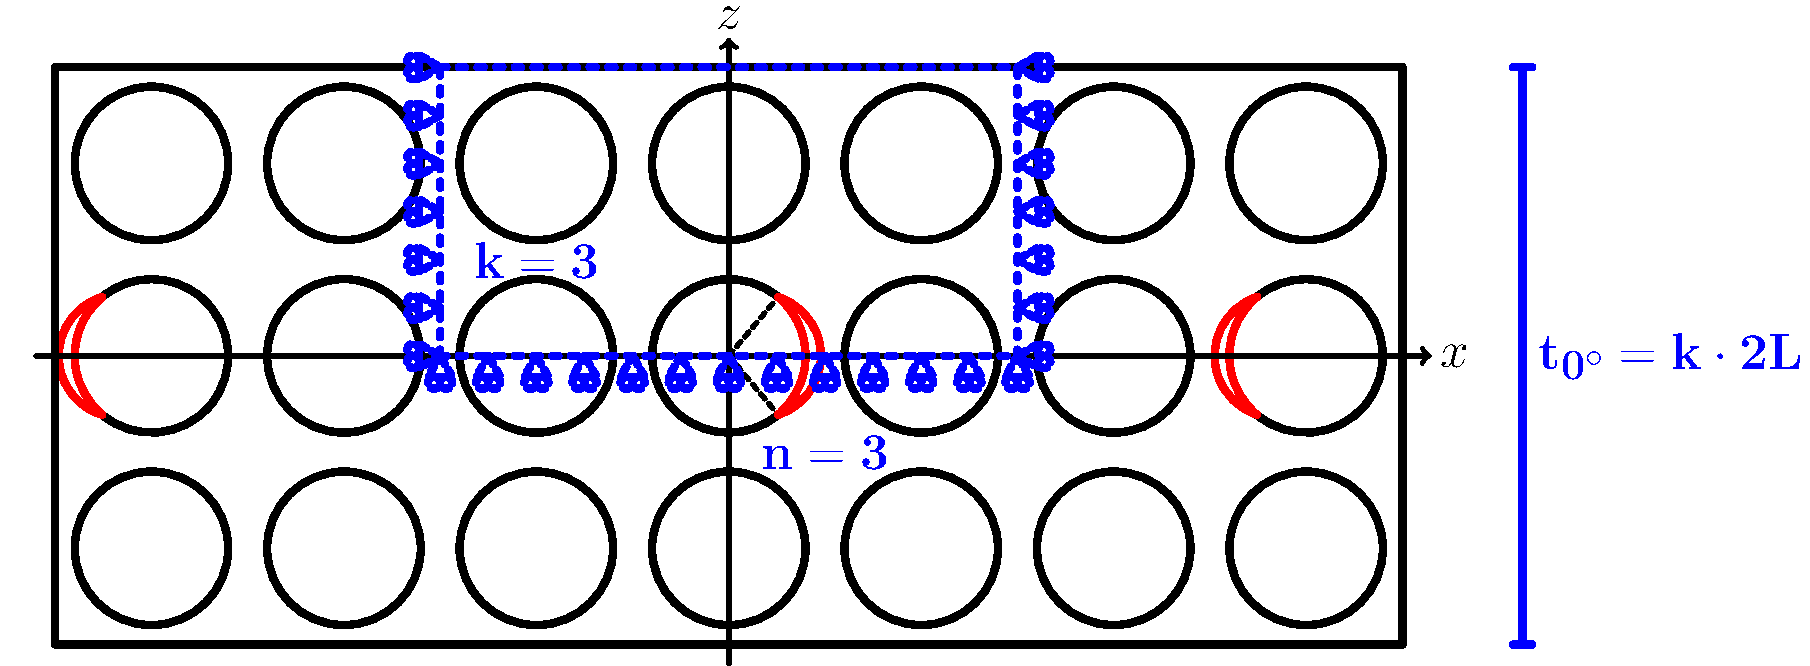
\includegraphics[width=0.4\textwidth]{thickPlyUD.pdf}}}\quad 
    \subfigure[$n\times k-coupling$]{\label{fig:rves-b}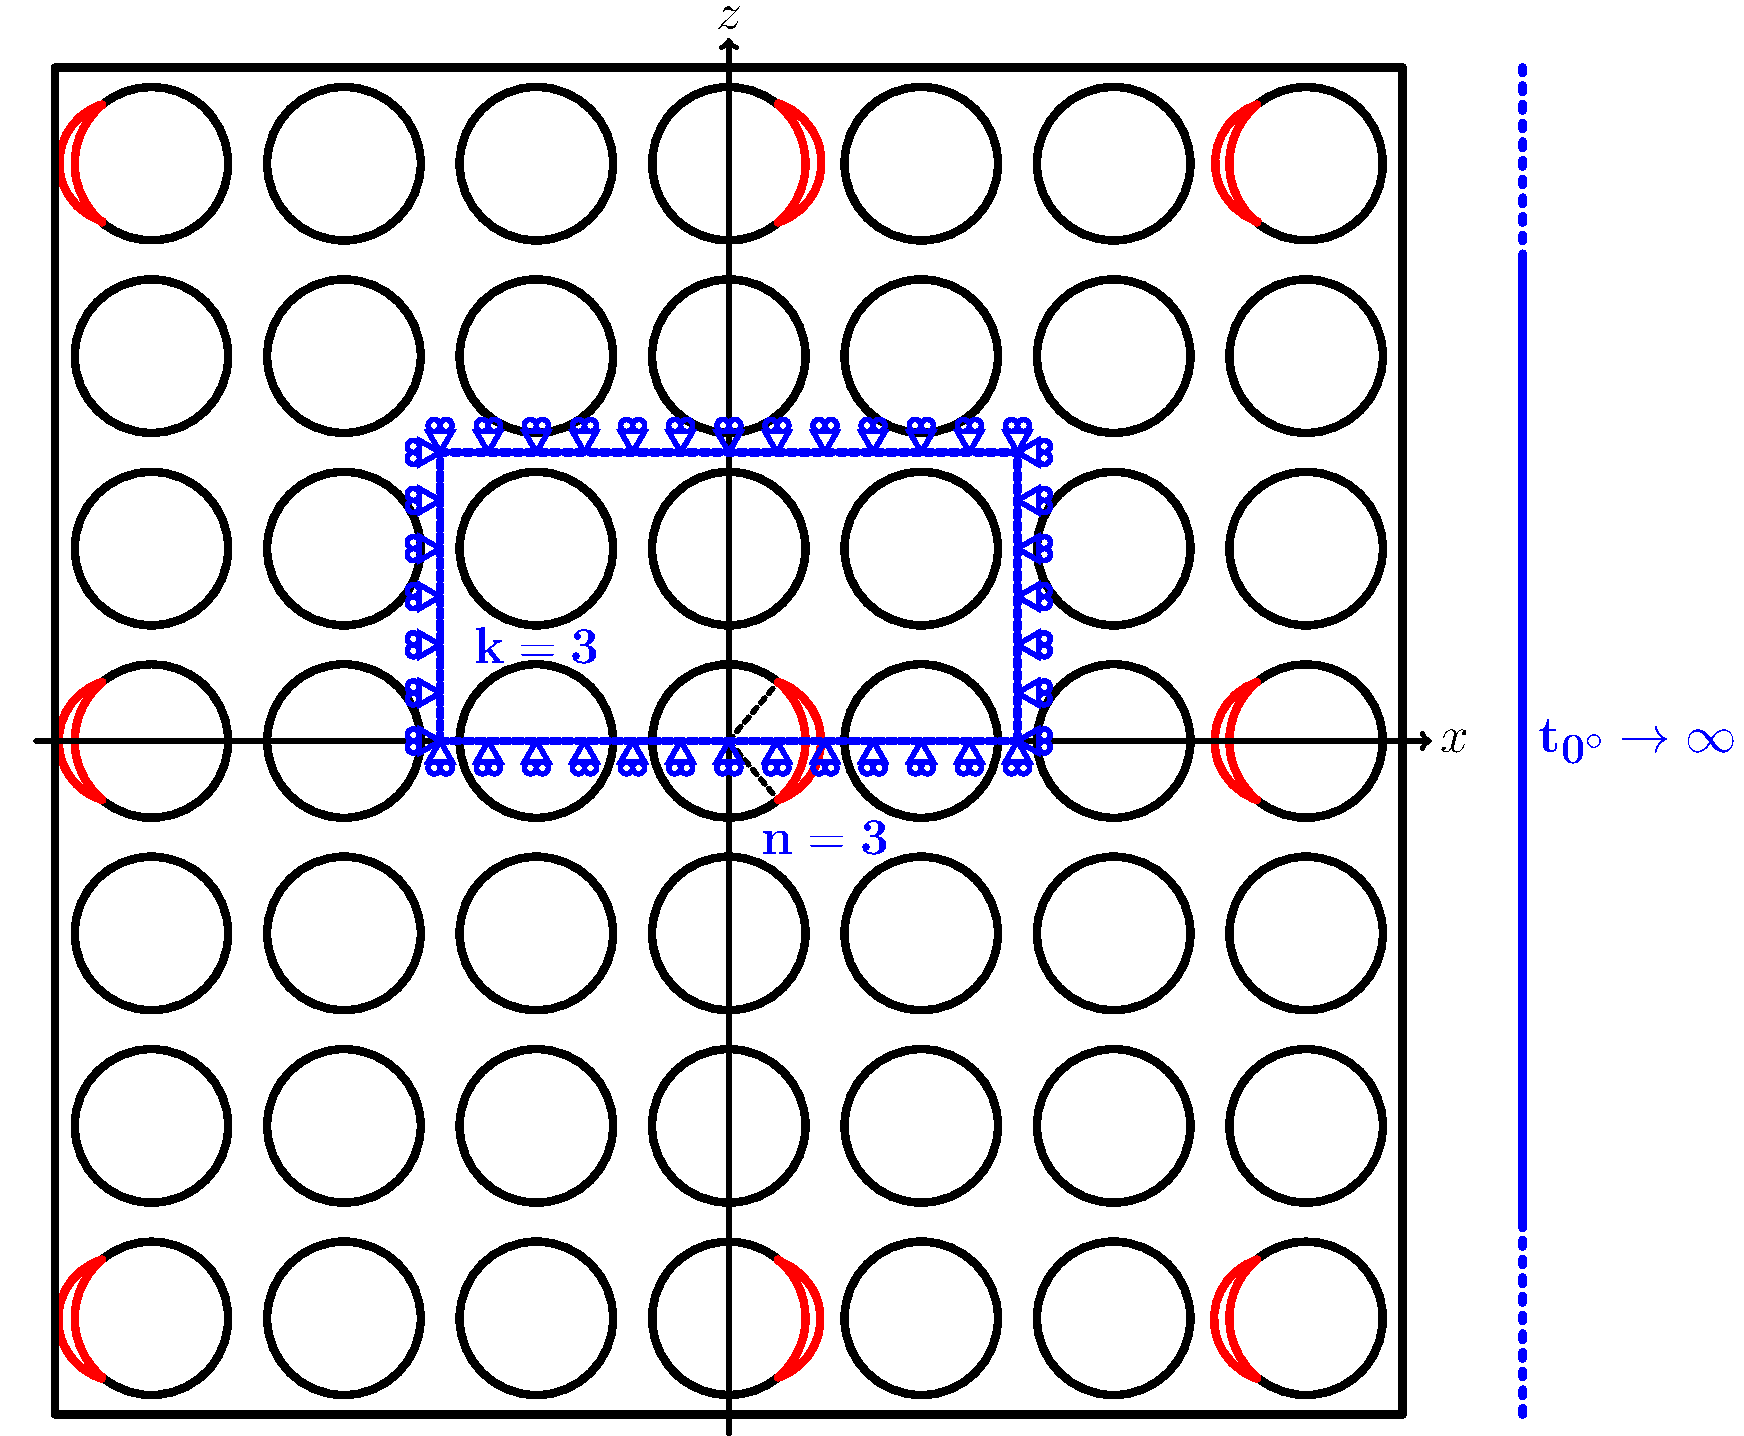
\includegraphics[width=0.4\textwidth]{coupling.pdf}}\\
    \subfigure[$n\times k-asymm$]{\label{fig:rves-c}\raisebox{0.0275\textheight}{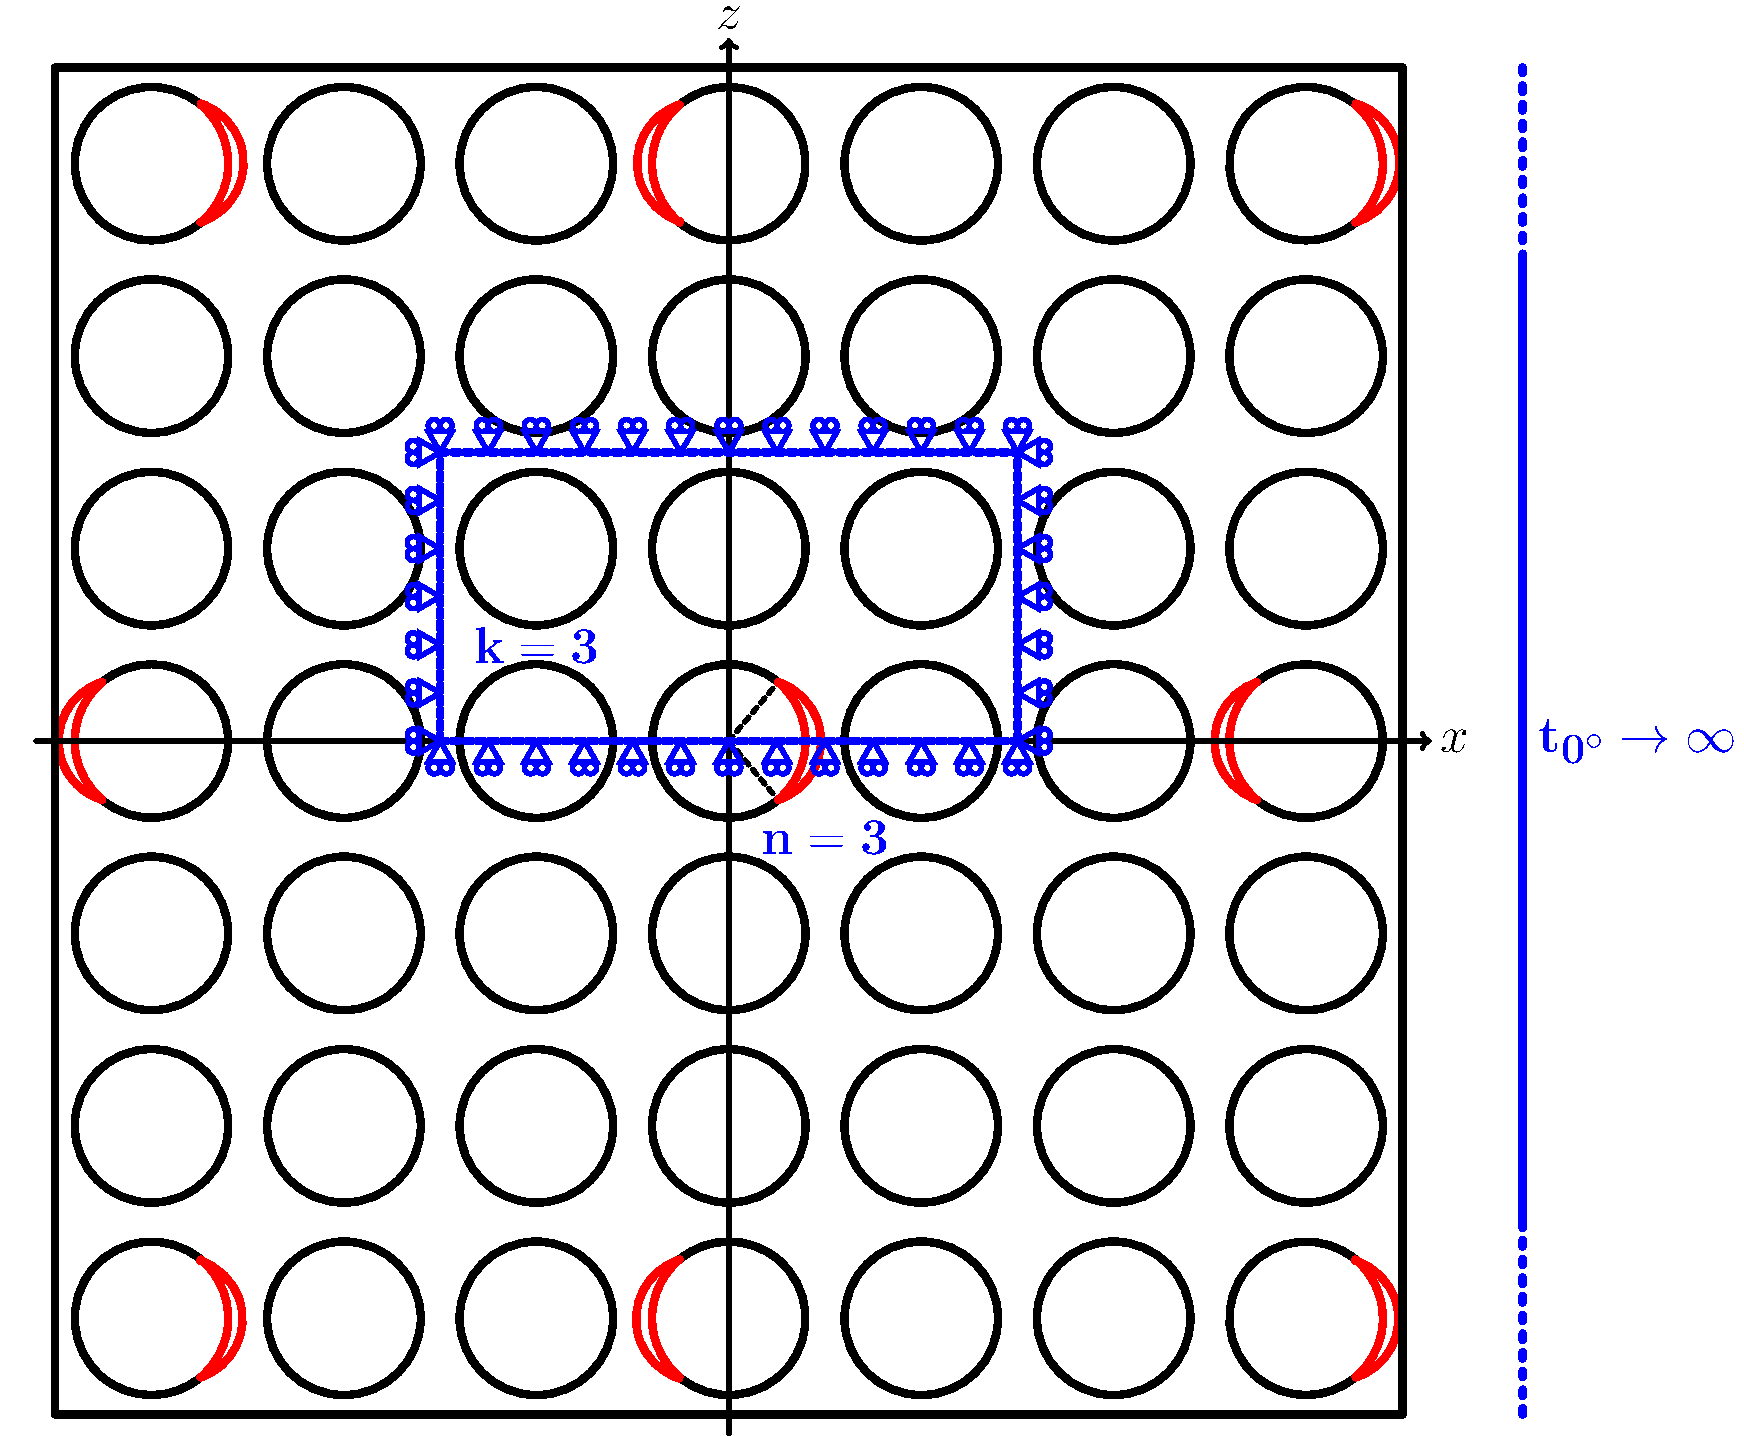
\includegraphics[width=0.4\textwidth]{asymm.pdf}}}\quad
    \subfigure[$n\times k-m\times t_{90^{\circ}}$]{\label{fig:rves-d}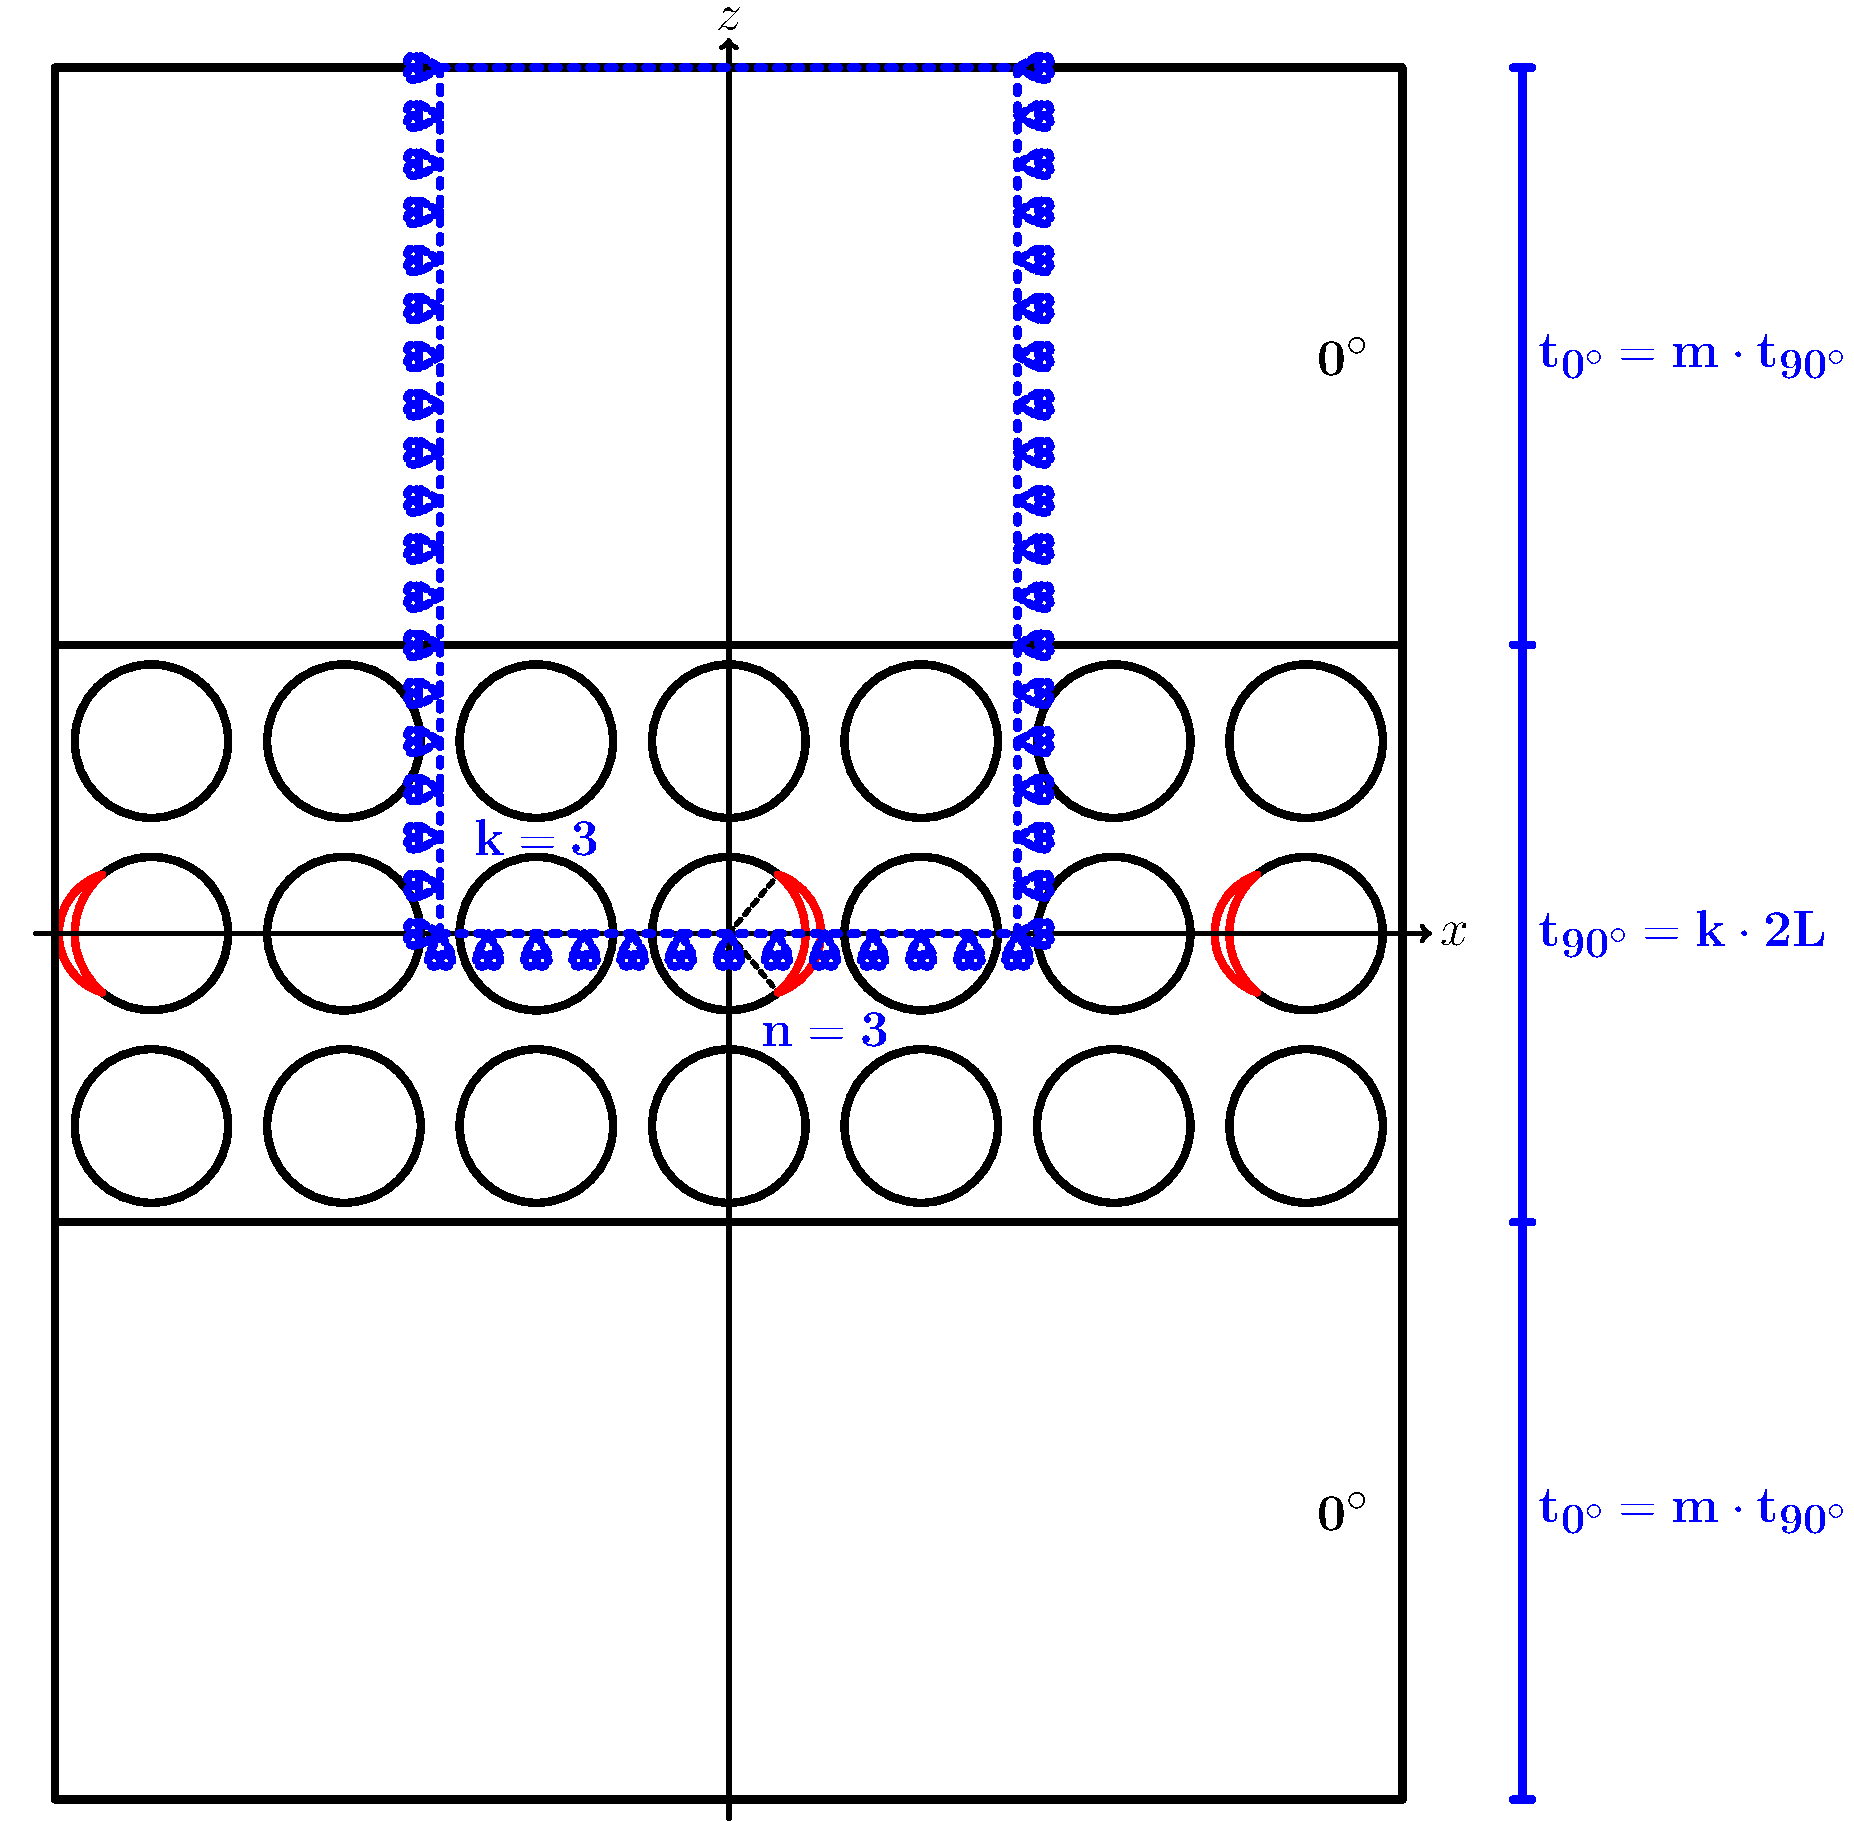
\includegraphics[width=0.4\textwidth]{ThickPlyCP.pdf}}
\caption{Composite RVEs and corresponding RUCs analyzed.}\label{fig:rves}
\end{figure}

Every RUC is symmetric with respect to the horizontal ($x$) direction, thus only half of it is modeled in the FE solution through the use of symmetry boundary conditions on the bottom side. Conditions of coupling of the horizontal displacement are applied on the left and right side, to model the repetition of the RUC along the horizontal direction. A tensile load is applied on the right and left side in the form of displacement $\bar{u}_{x}=\pm\bar{\varepsilon}_{x}nL$ with $\bar{\varepsilon}_{x}=1\%$. The debond has a size of $2\Delta\theta$ (see Figure~\ref{fig:ruc}), with $\Delta\theta\geq0$ ($\Delta\theta=0$ is the case of no damage at all). For large debonds ($\Delta\theta\geq 60^{\circ}-80^{\circ}$), a region called \emph{contact zone}, of size $\Delta\Phi$ to be determined by the solution itself, appears at the crack tip. Correct resolution of this behavior requires the imposition of conditions of non-interpenetration of the crack faces. Crack face contact is assumed to be frictionless.

\begin{figure}[!h]
\centering
        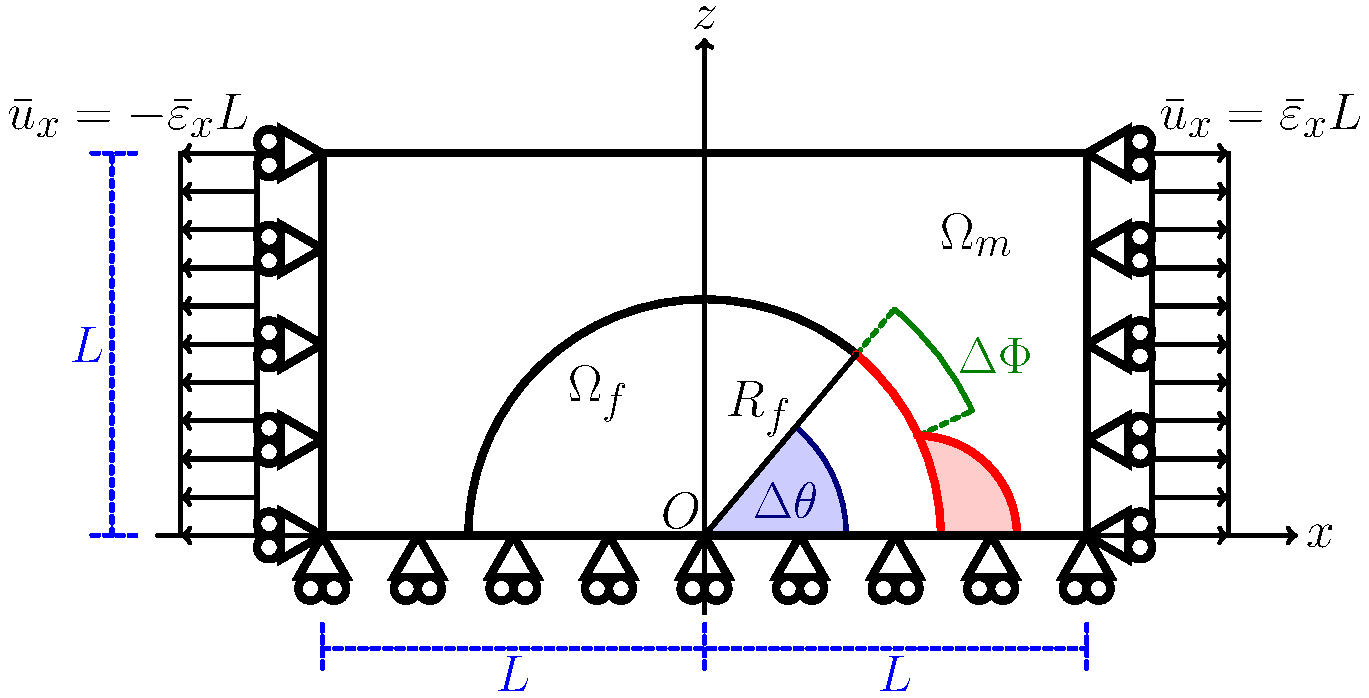
\includegraphics[height=0.15\textheight]{RUC.pdf}
\caption{One-fiber unit cell and main parameters characterizing the debonding process.}\label{fig:ruc}
\end{figure}

The FE solution is obtained using Abaqus~\cite{abq12} using second order, 2D, plane strain triangular (CPE6) and rectangular (CPE8) elements. To accurately resolve the singularity at the crack tip, a regular mesh of only rectangular elements is used with almost unitary aspect ratio and angular size $\delta=0.05^{\circ}$. The crack faces are represented as element-based surfaces with frictionless small-sliding contact pair interaction.

\begin{figure}[!h]
\centering
        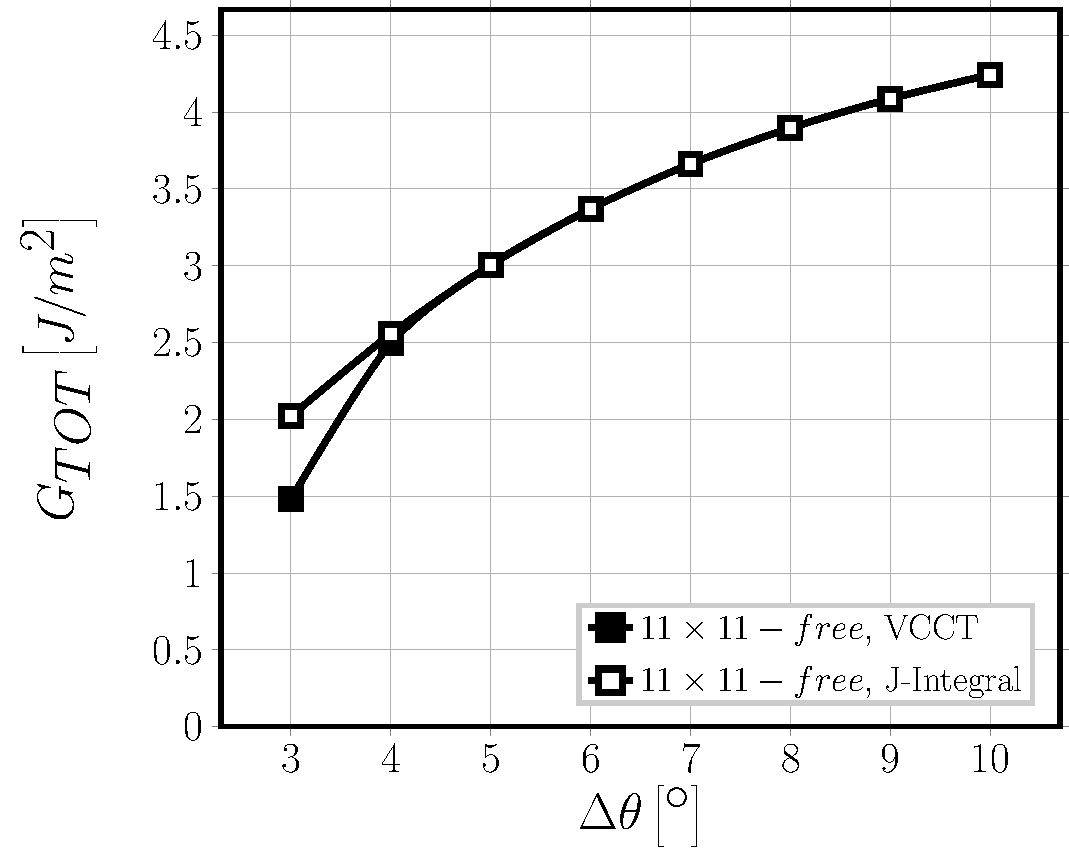
\includegraphics[height=0.2\textheight]{vf60-G-methodsaccuracy.pdf}
\caption{Total ERR of $11\times11-free$ evaluated respectively with the VCCT and the J-integral.}\label{fig:errerror}
\end{figure}

Total ERR is underestimated, due to the high $\frac{\delta}{\Delta\theta}$ ratio, with the Virtual Crack Closure Technique (VCCT)~\cite{Krueger2004} for very small debonds (see Figure~\ref{fig:errerror}), where it is dominated by Mode I. Thus, for $\Delta\theta<10^{\circ}$, $G_{TOT}$ is evaluated using the J-integral~\cite{Rice1968}, $G_{II}$ with the VCCT and $G_{I}=G_{TOT}-G_{II}$; for $\Delta\theta\geq10^{\circ}$ only the VCCT is used. Validation of the model is performed with respect to BEM results of~\cite{Paris2007,Sandino2016}; the order of accuracy of the results is discussed in~\cite{DiStasio2019}.

\begin{figure}[!hp]
\centering
    \subfigure[Radial stress $\sigma_{rr}$]{\label{fig:stress-a}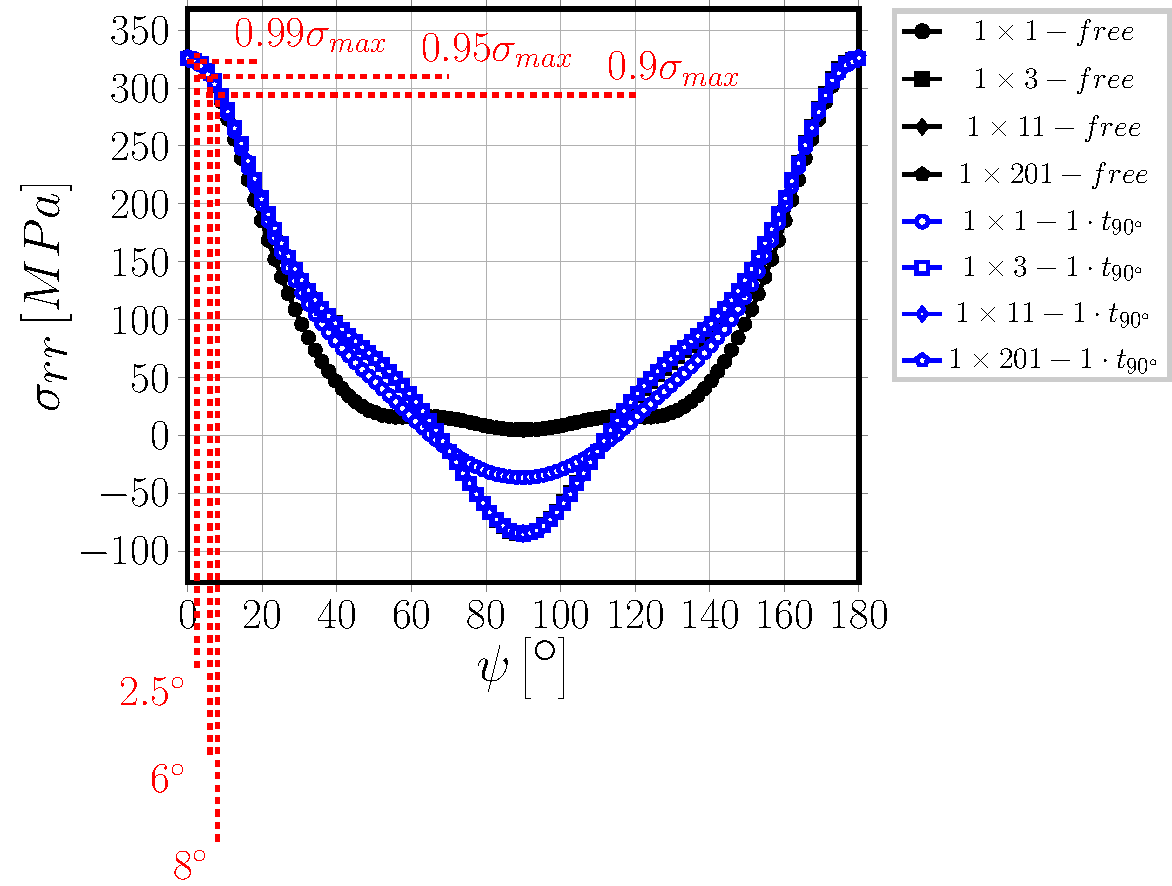
\includegraphics[height=0.2\textheight]{vf60-nodamage-sigmar.pdf}}\  
    \subfigure[Shear stress $\tau_{r\psi}$]{\label{fig:stress-b}\raisebox{0.04\textheight}{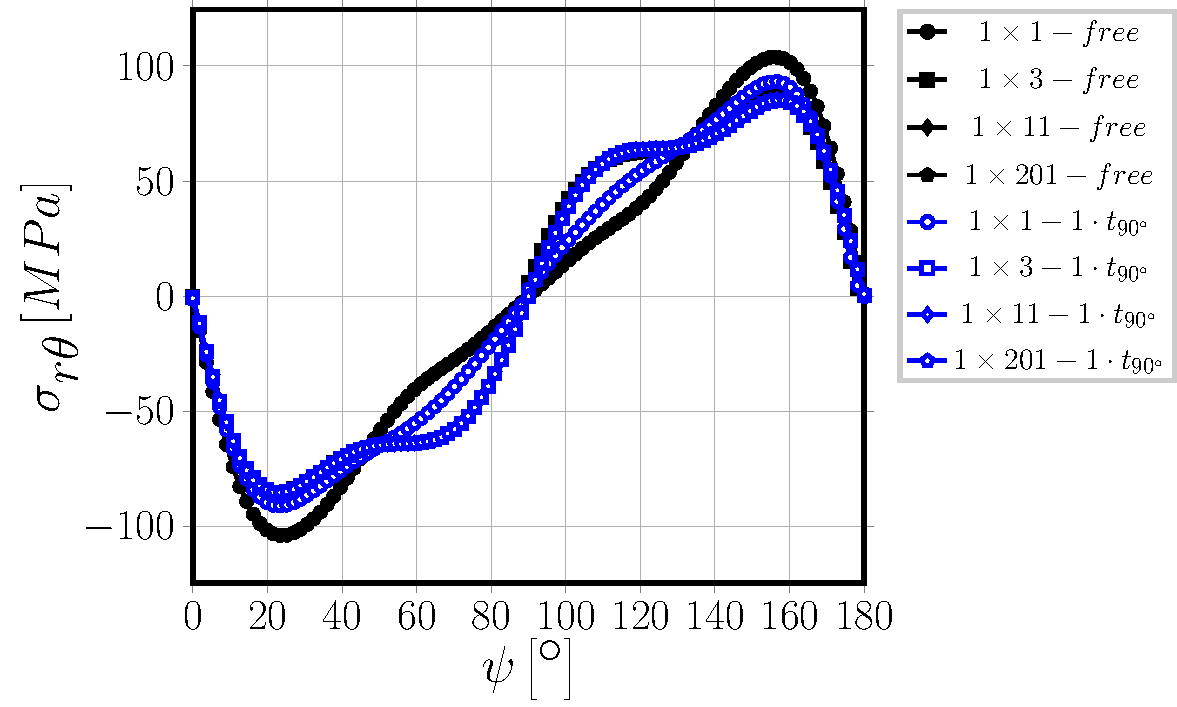
\includegraphics[height=0.16\textheight]{vf60-nodamage-taurt.pdf}}}\\
    \subfigure[Local Hydrostatic Stress (LHS), neglecting $\sigma_{yy}$, $\sigma_{LHS,2D}$.]{\label{fig:stress-c}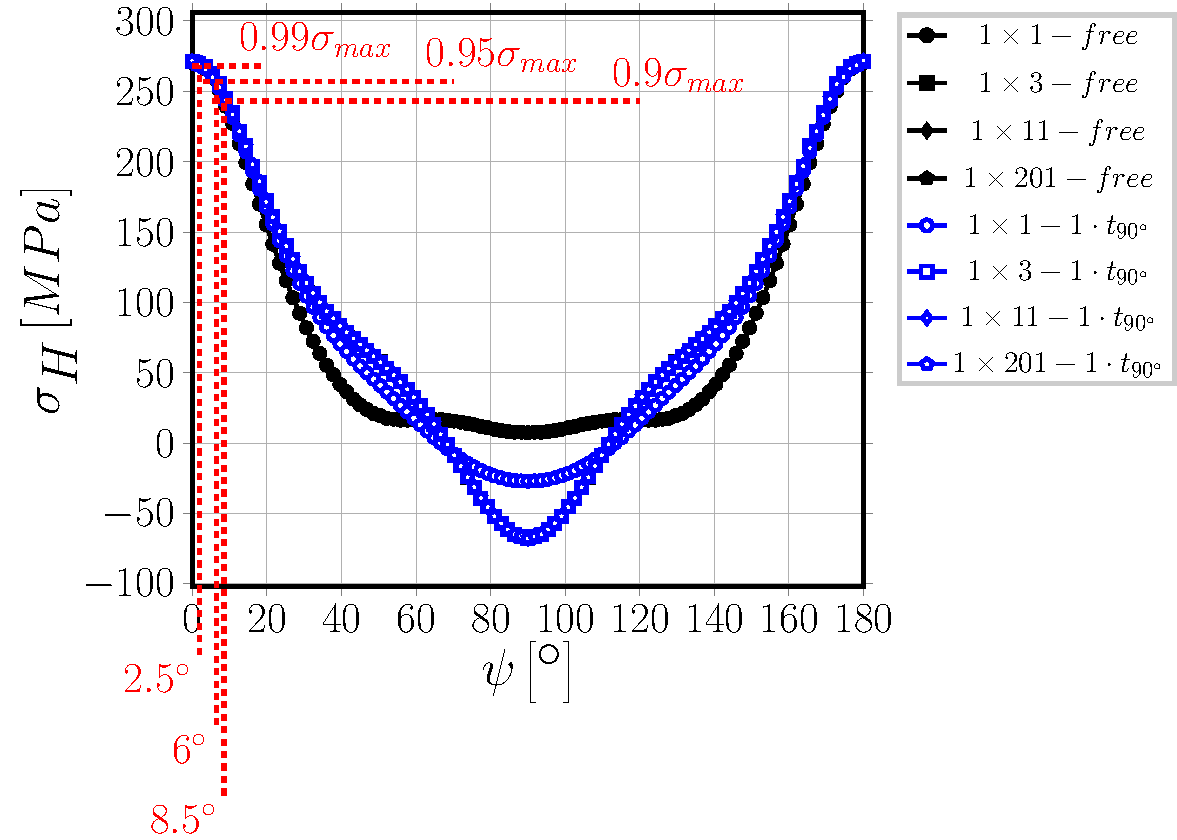
\includegraphics[height=0.2\textheight]{vf60-nodamage-p2D.pdf}}\ 
    \subfigure[Local Hydrostatic Stress (LHS), considering $\sigma_{yy}$, $\sigma_{LHS,3D}$.]{\label{fig:stress-d}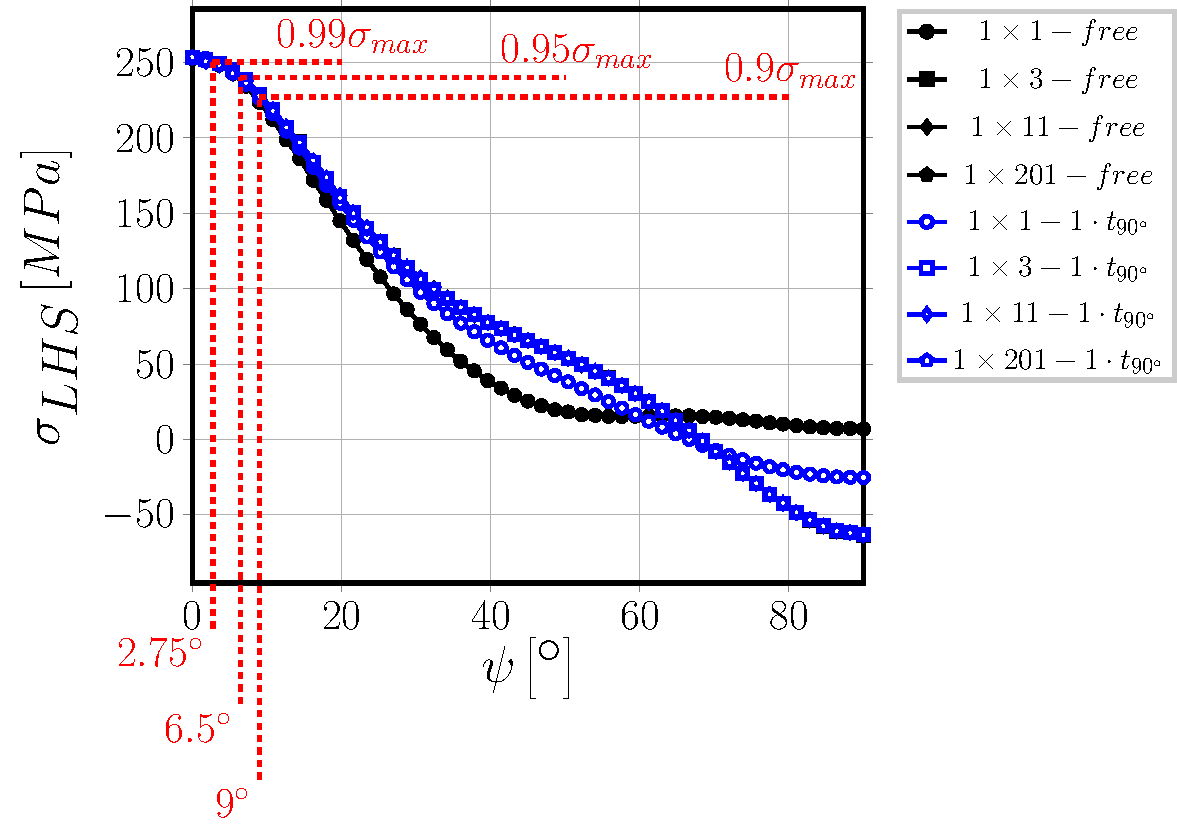
\includegraphics[height=0.2\textheight]{vf60-nodamage-p3D.pdf}}
    \subfigure[Local von Mises stress, neglecting $\sigma_{yy}$, $\sigma_{vM,2D}$.]{\label{fig:stress-e}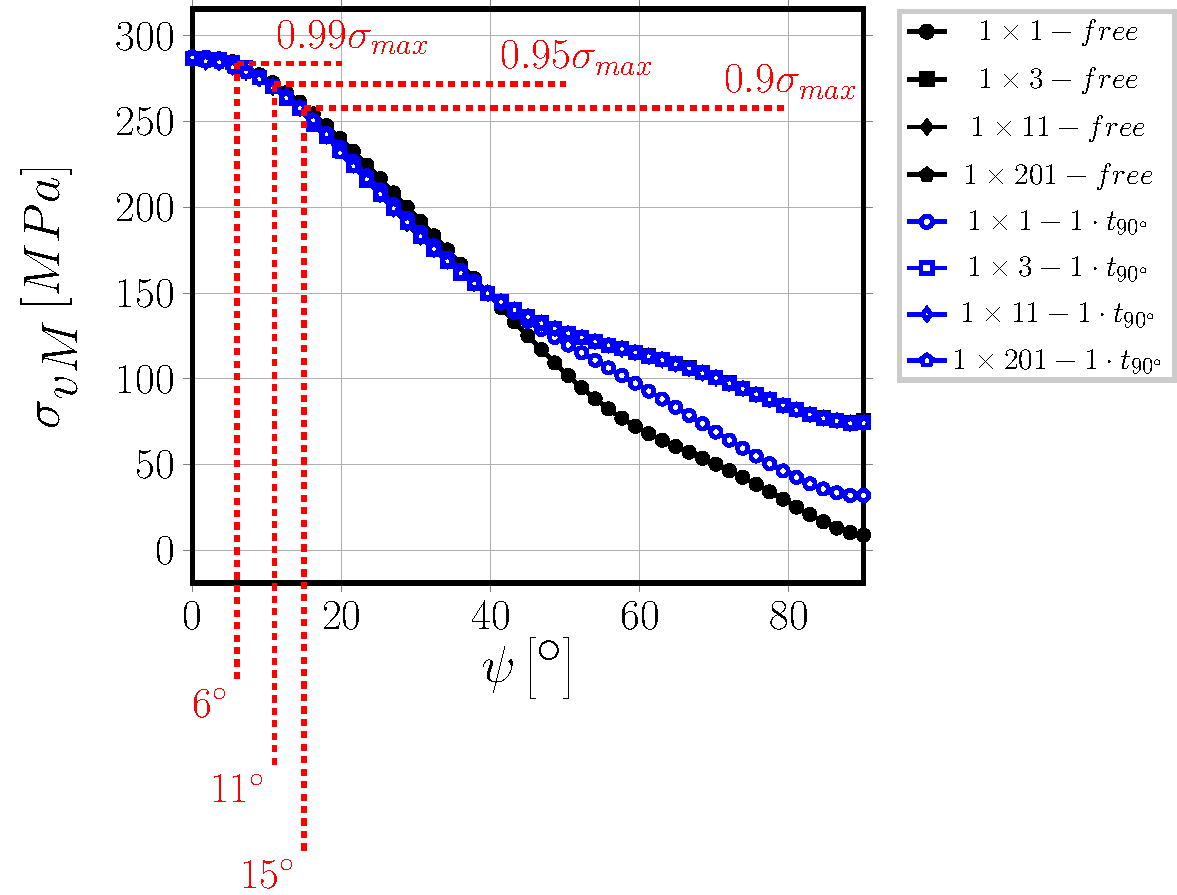
\includegraphics[height=0.2\textheight]{vf60-nodamage-vM2D.pdf}}\ 
    \subfigure[Local von Mises stress, considering $\sigma_{yy}$, $\sigma_{vM,3D}$.]{\label{fig:stress-f}\raisebox{0.04\textheight}{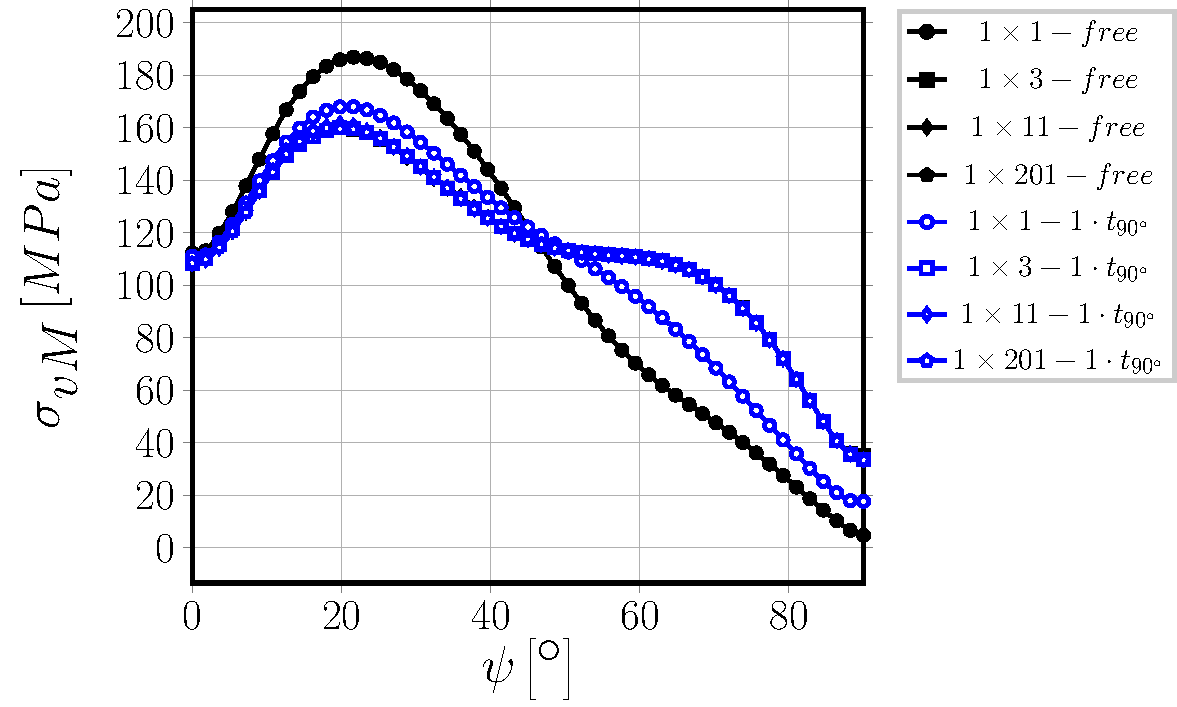
\includegraphics[height=0.16\textheight]{vf60-nodamage-vM3D.pdf}}}
    \subfigure[Local Maximum Principal Stress (LMPS), neglecting $\sigma_{yy}$, $\sigma_{LMPS,2D}$.]{\label{fig:stress-g}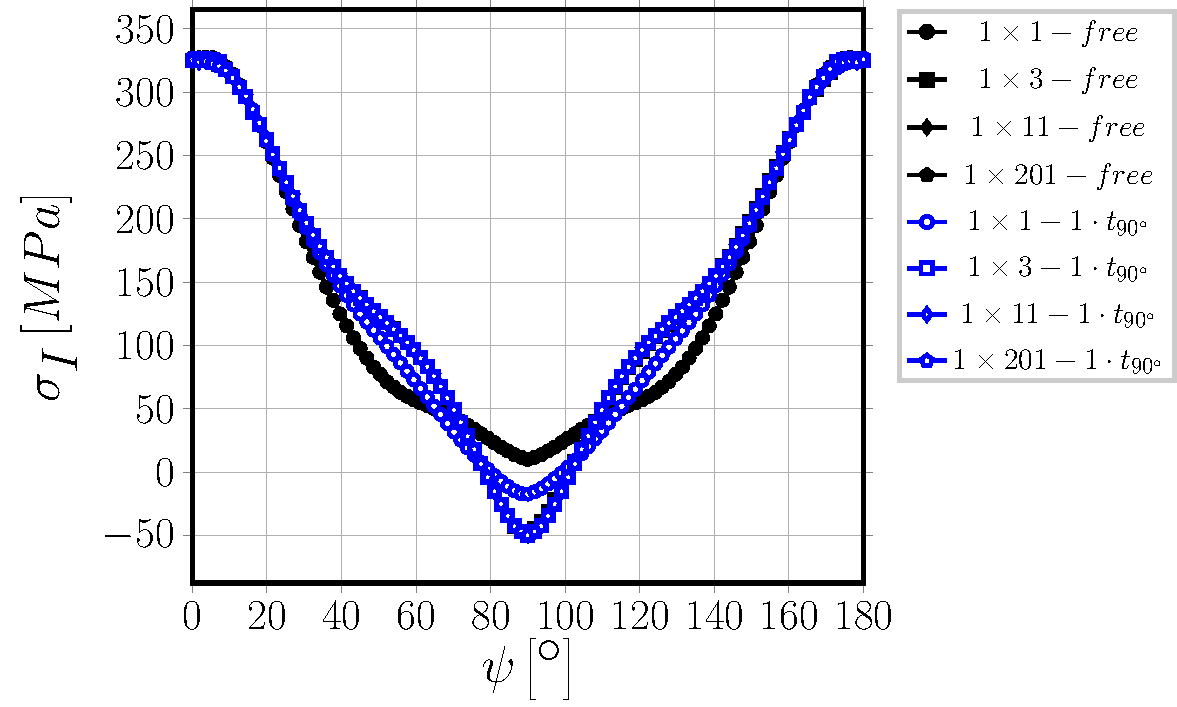
\includegraphics[height=0.2\textheight]{vf60-nodamage-sigmaI2D.pdf}}\ 
    \subfigure[Local Maximum Principal Stress (LMPS), considering $\sigma_{yy}$, $\sigma_{LMPS,3D}$.]{\label{fig:stress-h}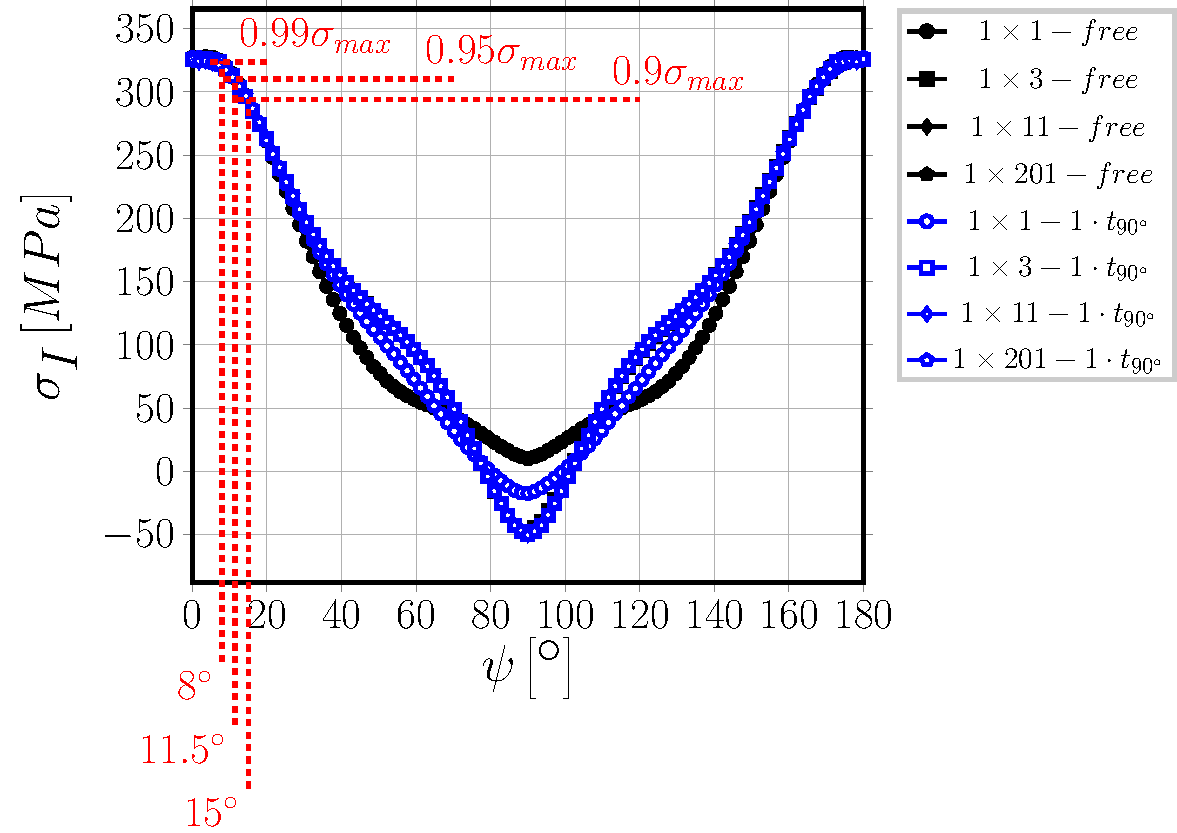
\includegraphics[height=0.2\textheight]{vf60-nodamage-sigmaI3D.pdf}}
\caption{Stress distribution at the fiber/matrix interface in the absence of damage with respect to angular coordinate $\psi$; applied strain $\bar{\varepsilon}_{x}=1\%$.}\label{fig:stress}
\end{figure}

\section{STRESS-BASED ANALYSIS OF DEBOND INITIATION ($\Delta\theta=0^{\circ}$)}\label{sec:stress}

In this section, we assume stress-based debond initiation at the undamaged fiber/matrix interface. Thus, we analyze the distribution of stresses at the fiber/matrix interface in models $1\times k-free$ and $1\times k-1\cdot t_{90^{\circ}}$ with $k=1,3,11,201$, $\Delta\theta=0^{\circ}$ (i.e. the undamaged case) and $\bar{\varepsilon}_{x}=1\%$. Some selected stress components are presented, based on their relevance in previous studies on debond initiation and growth: the radial $\sigma_{rr}$ and shear $\tau_{r\psi}$ stress~\cite{Mantic2009} (Fig.~\ref{fig:stress-a} and Fig.~\ref{fig:stress-b}), the Local Hydrostatic Stress (LHS, following the notation of~\cite{Carraro2016}) $\sigma_{LHS}$~\cite{Asp1996a,Asp1996b} (Fig.~\ref{fig:stress-c} and Fig.~\ref{fig:stress-d}), the local von Mises stress $\sigma_{vM}$~\cite{Canal2012}  (Fig.~\ref{fig:stress-e} and Fig.~\ref{fig:stress-f}), the Local Maximum Principal Stress (LMPS, following the notation of~\cite{Carraro2016}) $\sigma_{LMPS}$~\cite{Carraro2014}  (Fig.~\ref{fig:stress-g} and Fig.~\ref{fig:stress-h}). In plane strain conditions imply that there exists an out-of-plane axial component of the stress ($\sigma_{yy}$ in our notation): in order to study the importance of this out-of-plane component (tri-axial stress state, see~\cite{Asp1995}), $\sigma_{LHS}$, $\sigma_{vM}$ and $\sigma_{LMPS}$ are evaluated both neglecting (index $2D$) and considering it (index $3D$).\\
It is possible to observe that:
\vspace{-5pt}
\begin{enumerate}
\itemsep-0.5pt
\item for all stresses reported in Fig.~\ref{fig:stress}, no significant difference is present between the different RUCs for $\psi\leq10^{\circ}$;
\item for all stresses reported in Fig.~\ref{fig:stress}, no difference can be observed by increasing $k$ when $k\geq3$;
\item for all stresses reported in Fig.~\ref{fig:stress}, no difference can be observed between $1\times  k-free$ and $1\times  k-1\cdot t_{90^{\circ}}$ for $k\geq3$;
\item at $\psi=0^{\circ}$ (i.e. the intersection between fiber/matrix interface and horizontal axis); the shear stress $\tau_{r\psi}$ (Fig.~\ref{fig:stress-b}) is $0$ while the radial stress $\sigma_{rr}$ (Fig.~\ref{fig:stress-a}) is at its maximum;
\item comparison of Fig.~\ref{fig:stress-c} with Fig.~\ref{fig:stress-d} shows that the out-of-plane stress $\sigma_{yy}$ has only a marginal effect on the local hydrostatic stress $\sigma_{LHS}$: the distribution remains the same, while the peak value is reduced from $270\ \left[MPa\right]$ in Fig.~\ref{fig:stress-c} to $250\ \left[MPa\right]$ in Fig.~\ref{fig:stress-d} by considering $\sigma_{yy}$;
\item comparison of Fig.~\ref{fig:stress-e} with Fig.~\ref{fig:stress-f} shows a remarkable effect of the out-of-plane stress $\sigma_{yy}$ on the von Mises stress: if $\sigma_{yy}$ is neglected, $\sigma_{vM}$ presents a maximum of $287\ \left[MPa\right]$ at $\psi=0^{\circ}$, slightly higher than the value of $\sigma_{LHS}$ (neglecting $\sigma_{yy}$) of $270\ \left[MPa\right]$ at $\psi=0^{\circ}$; if $\sigma_{yy}$ is considered, the peak value of $\sigma_{vM}$ is shifted to $\psi\sim20^{\circ}$ and reduced to $186\ \left[MPa\right]$ while at $\psi=0^{\circ}$ $\sigma_{vM}$ is reduced to $\sim110\ \left[MPa\right]$, significantly lower than $\sigma_{LHS}=250\ \left[MPa\right]$ at $\psi=0^{\circ}$ (considering $\sigma_{yy}$);
\item comparison of Fig.~\ref{fig:stress-g} with Fig.~\ref{fig:stress-g} shows that the Local Maximum Principal Stress is practically unaffected by the out-of-plane stress $\sigma_{yy}$;
\item $\sigma_{rr}$, $\sigma_{LHS,2D}$, $\sigma_{LHS,3D}$, $\sigma_{vM,2D}$, $\sigma_{LMPS,2D}$ and $\sigma_{LMPS,3D}$ all reach their peak value at $0^{\circ}$ and $180^{\circ}$ and decrease to $99\%$ the peak value between $2^{\circ}$ and $8^{\circ}$, to $95\%$ the peak value between $6^{\circ}$ and $12^{\circ}$ and to $90\%$ the peak value between $8^{\circ}$ and $15^{\circ}$ from the occurrence of the maximum.
\end{enumerate}
\vspace{-5pt}
Based on the previous considerations, it is reasonable to assume that a stress-based criterion would predict, irrespectively of the specific criterion chosen, the onset of an interface crack at $0^{\circ}$ or $180^{\circ}$ with an initial size at least comprised in the range $2^{\circ}-8^{\circ}$ ($1\%$ margin) and likely in the range $6^{\circ}-12^{\circ}$ ($5\%$ margin). It is worth to point out that, in the case of a linear elastic solution as the one presented here, the stresses at the fiber/matrix interface for a different value of the applied strain $\bar{\varepsilon}_{x}$ will change in magnitude but will keep the same functional form and relative magnitude with respect to each other. Thus, the considerations made so far, based on the relative magnitude of stresses and their rate of decrease from the peak value, will apply at any other strain level.

\section{ENERGY-BASED ANALYSIS OF DEBOND PROPAGATION}

In the previous section, we assumed stress-based debond initiation. We now assume that, once an initial debond is formed of a size in the range predicted in the previous section ($\Delta\theta_{0}\sim2^{\circ}-12^{\circ}$), the debond will grow unstably~\cite{Correa2016} according to an energy-based criterion of the form~\cite{Hutchinson1991,Mantic2009}:

\begin{equation}\label{eq:propcrit}
G_{TOT}\geq G_{c}=G_{Ic}\left(1+\tan^{2}\left(\left(1-\lambda\right)\Psi_{G}\right)\right),\quad\Psi_{G}=tan^{-1}\left(\sqrt{\frac{G_{II}}{G_{I}}}\right),
\end{equation}

where $\Psi_{G}$ is the energy-based phase angle, $G_{TOT}$ is the total ERR, $G_{c}$ is the critical ERR, $G_{Ic}$ is the Mode I critical ERR (material property) and $\lambda$ the mode mixity sensitivity parameter (material property, usually $0.2\leq\lambda\leq0.35$)\footnote{$\lambda$ governs the influence of mode ratio $\frac{G_{II}}{G_{I}}$ on $G_{c}$ such that: for $\lambda=1$, $G_{c}=G_{Ic}$; for $\lambda=0$, $G_{c}=G_{Ic}\left(1+\frac{G_{II}}{G_{I}}\right)$.}. Given that debond propagation starts as soon as an initial debond is formed (in our model), the propagation criterion in Eq.~\ref{eq:propcrit} is satisfied for the initial debond size $\Delta\theta_{0}$. Thus, by calculating $G_{I}$, $G_{II}$ and $G_{TOT}$ and equating $G_{c}$ to $G_{TOT}$ in Eq.~\ref{eq:propcrit}, it is possible to estimate $G_{Ic}$ for different values of the initial debond size $\Delta\theta_{0}$ and of the parameter $\lambda$ (Figure~\ref{fig:GIc}). The estimation is performed using a restricted set of RUCs: $11\times 1-free$, $11\times 11-free$, $11\times 1-1\cdot t_{90^{\circ}}$ and $11\times 11-1\cdot t_{90^{\circ}}$, with $\bar{\varepsilon}_{x}=1\%$.

\begin{figure}[!h]
\centering
    \subfigure[$\lambda=0.3$]{\label{fig:GIc-a}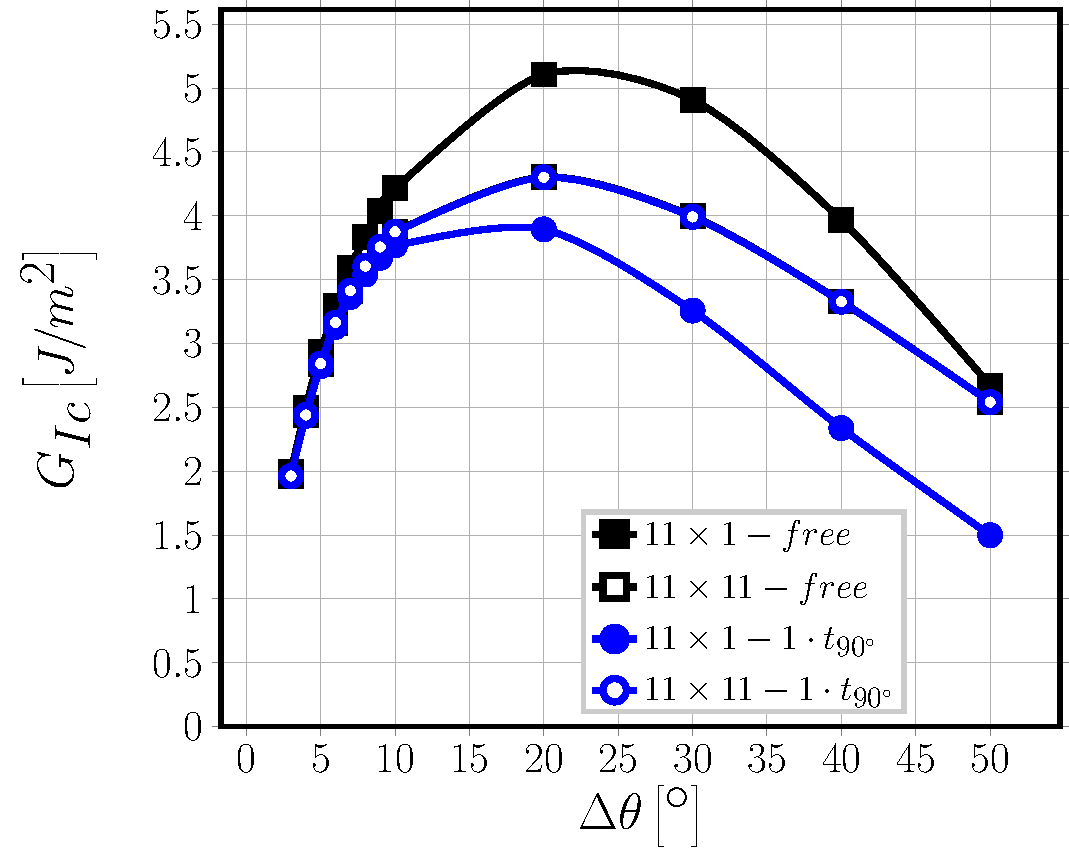
\includegraphics[height=0.25\textheight]{vf60-GIc-model.pdf}}\quad 
    \subfigure[$11\times 11-1\cdot t_{90^{\circ}}$]{\label{fig:GIc-b}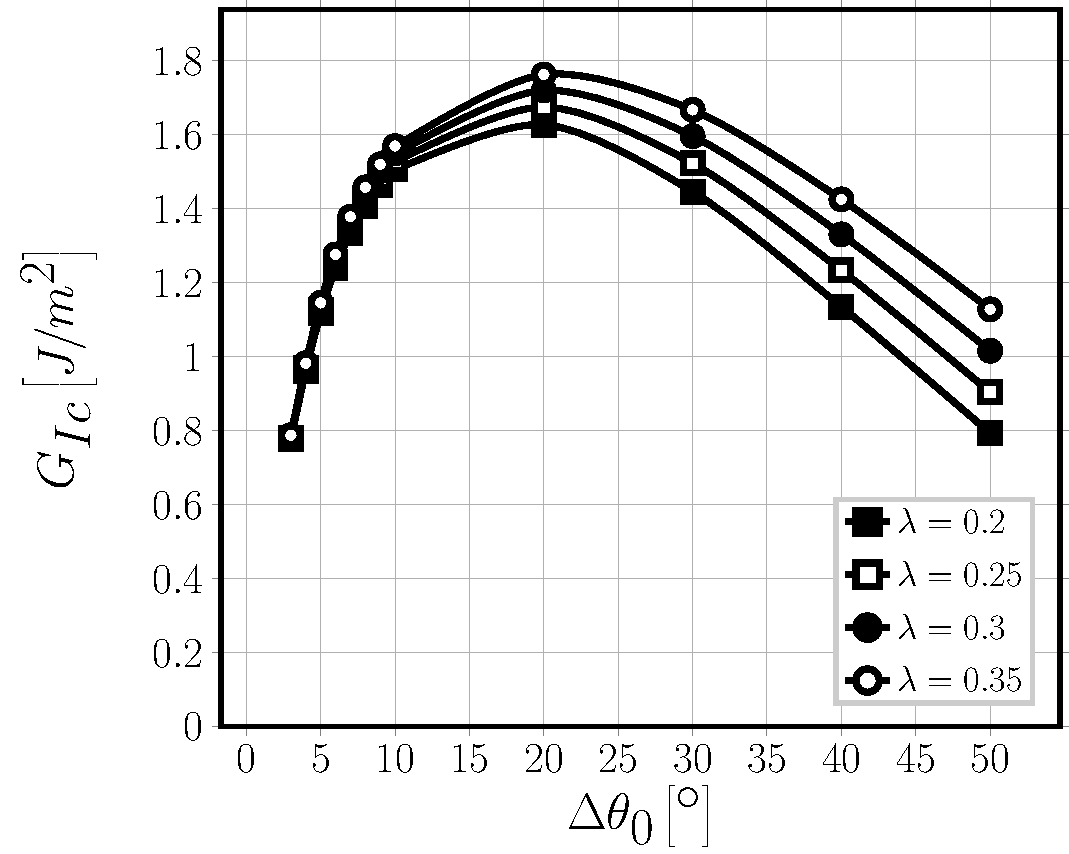
\includegraphics[height=0.25\textheight]{vf60-GIc-lambda.pdf}}
\caption{Estimated values of $G_{Ic}$ assuming different values of initial debond size, for different RUCs and varying $\lambda$.}\label{fig:GIc}
\end{figure}

Neither RUC configuration nor $\lambda$ affects $G_{Ic}$ significantly for small initial debond size, i.e $\Delta\theta_{0}<10^{\circ}$ (Figure~\ref{fig:GIc}), corresponding to the range of initial debond size determined in Section~\ref{sec:stress}. Observing Figure~\ref{fig:GIc}, we can assume a value of $G_{Ic}$ in the range $2-4.5\ \left[\frac{J}{m^{2}}\right]$, with $0.2\leq\lambda\leq0.35$. Notice that this estimate is based on calculations with $\bar{\varepsilon}_{x}=1\%$ and the value of $G_{Ic}$ will scale with $\bar{\varepsilon}_{x}$ according to $\frac{G_{Ic,\bar{\varepsilon}_{x,1}}}{G_{Ic,\bar{\varepsilon}_{x,2}}}=\left(\frac{\bar{\varepsilon}_{x,1}}{\bar{\varepsilon}_{x,2}}\right)^{2}$. Given that no dependence of $G_{Ic}$ on RUC type is observed for $\Delta\theta_{0}<10^{\circ}$, we can use $G_{Ic}\sim2-4.5\ \left[\frac{J}{m^{2}}\right]$ to estimate the expected maximum size of debonds in several other RUCs (Figure~\ref{fig:debondsize}), by evaluating $G_{c}$ according to Equation~\ref{eq:propcrit}. The expected maximum debond size $\Delta\theta_{max}$ is the value of $\Delta\theta$ such that 

\begin{equation}\label{eq:debmax}
G_{TOT}\left(\Delta\theta\geq\Delta\theta_{max}\right)\leq G_{c}\left(\Delta\theta\geq\Delta\theta_{max}\right).
\end{equation}

Notice that, although evaluated using $G_{I}$, $G_{II}$ and $G_{TOT}$ computed with $\bar{\varepsilon}_{x}=1\%$, the values of $\Delta\theta_{max}$ do not depend on $\bar{\varepsilon}_{x}$ as both sides in Equation~\ref{eq:debmax} scale with the applied strain by a factor $\left(\frac{\bar{\varepsilon}_{x,1}}{\bar{\varepsilon}_{x,2}}\right)^{2}$. If the procedure described in this section is applied using values of $G_{I}$, $G_{II}$ and $G_{TOT}$ computed with a different value of $\bar{\varepsilon}_{x}$, the estimated values of $\Delta\theta_{max}$ will be the same.

\begin{figure}[!htbp]
\centering
    \subfigure[$21\times 1-free$]{\label{fig:debondsize-a}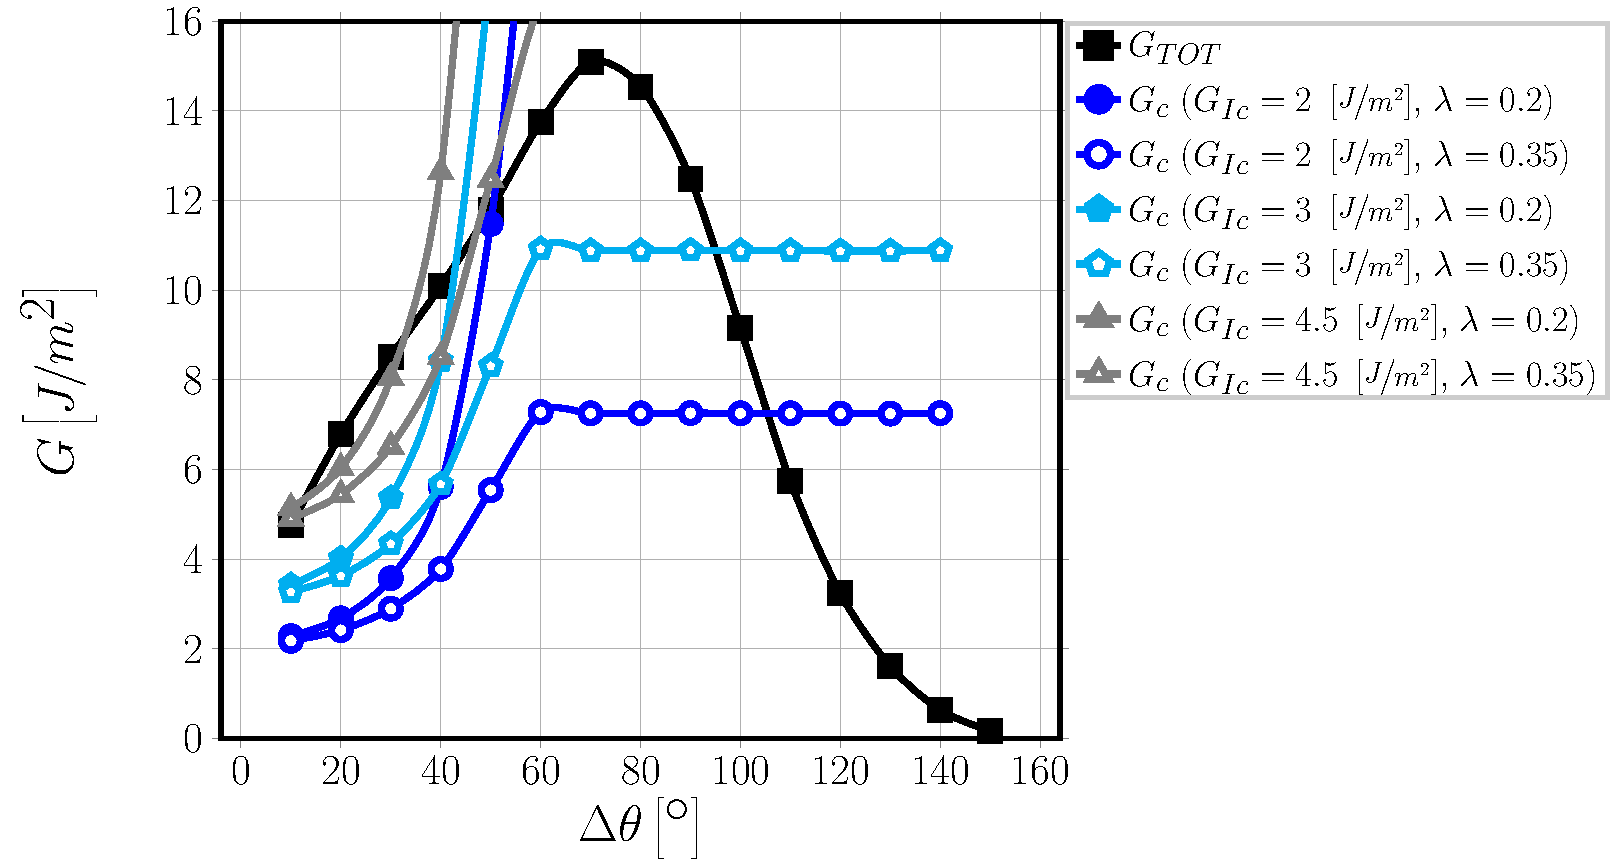
\includegraphics[width=0.45\textwidth]{vf60-dsize-S10A0.pdf}}\   
    \subfigure[$21\times 1-1\cdot t_{90^{\circ}}$]{\label{fig:debondsize-b}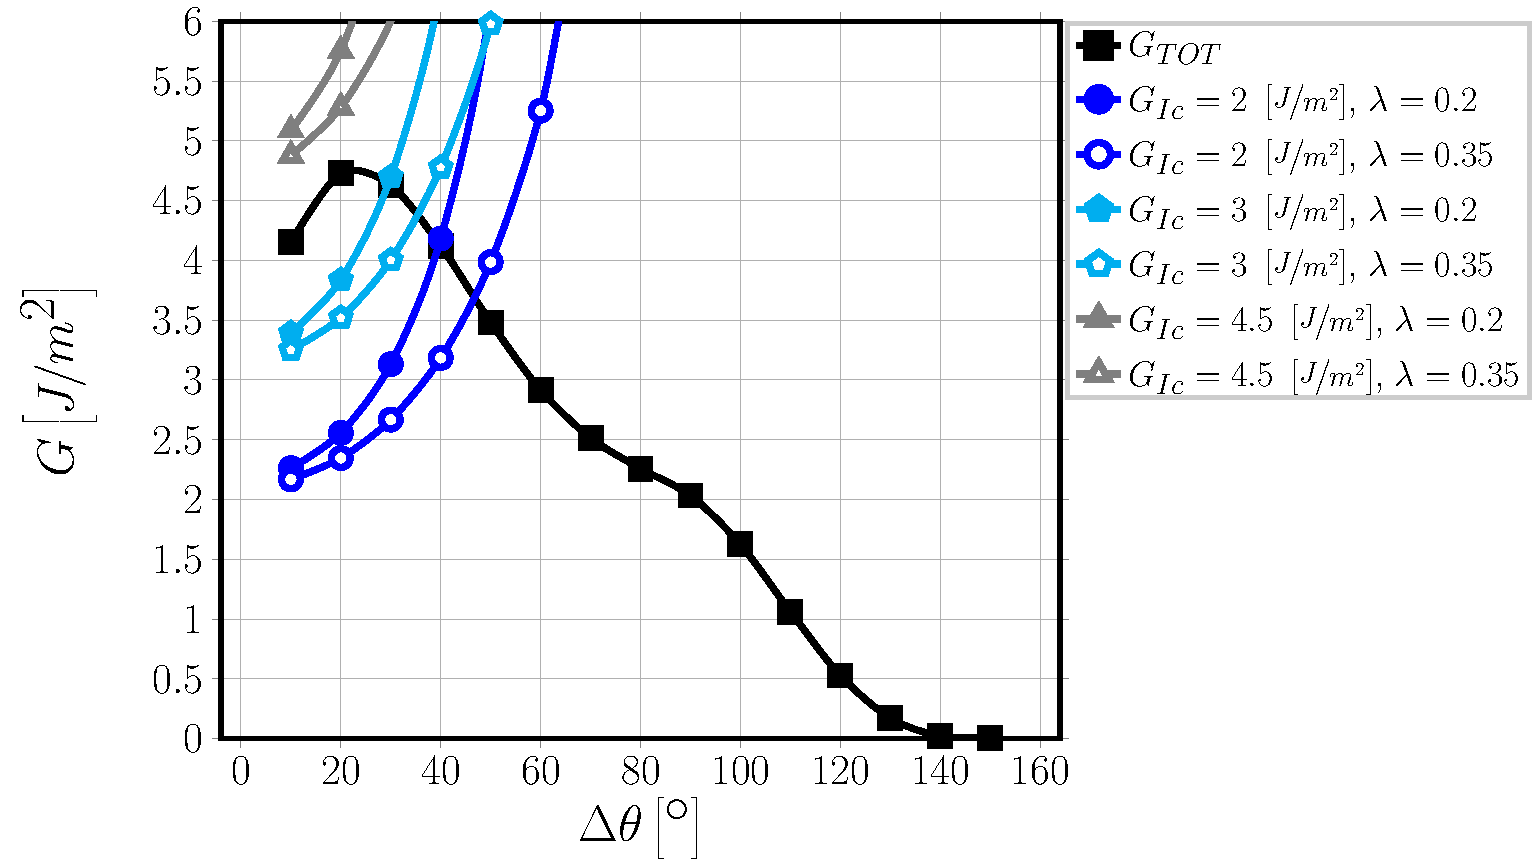
\includegraphics[width=0.45\textwidth]{vf60-dsize-S10A0T1.pdf}}\\
    \subfigure[$21\times 3-free$]{\label{fig:debondsize-c}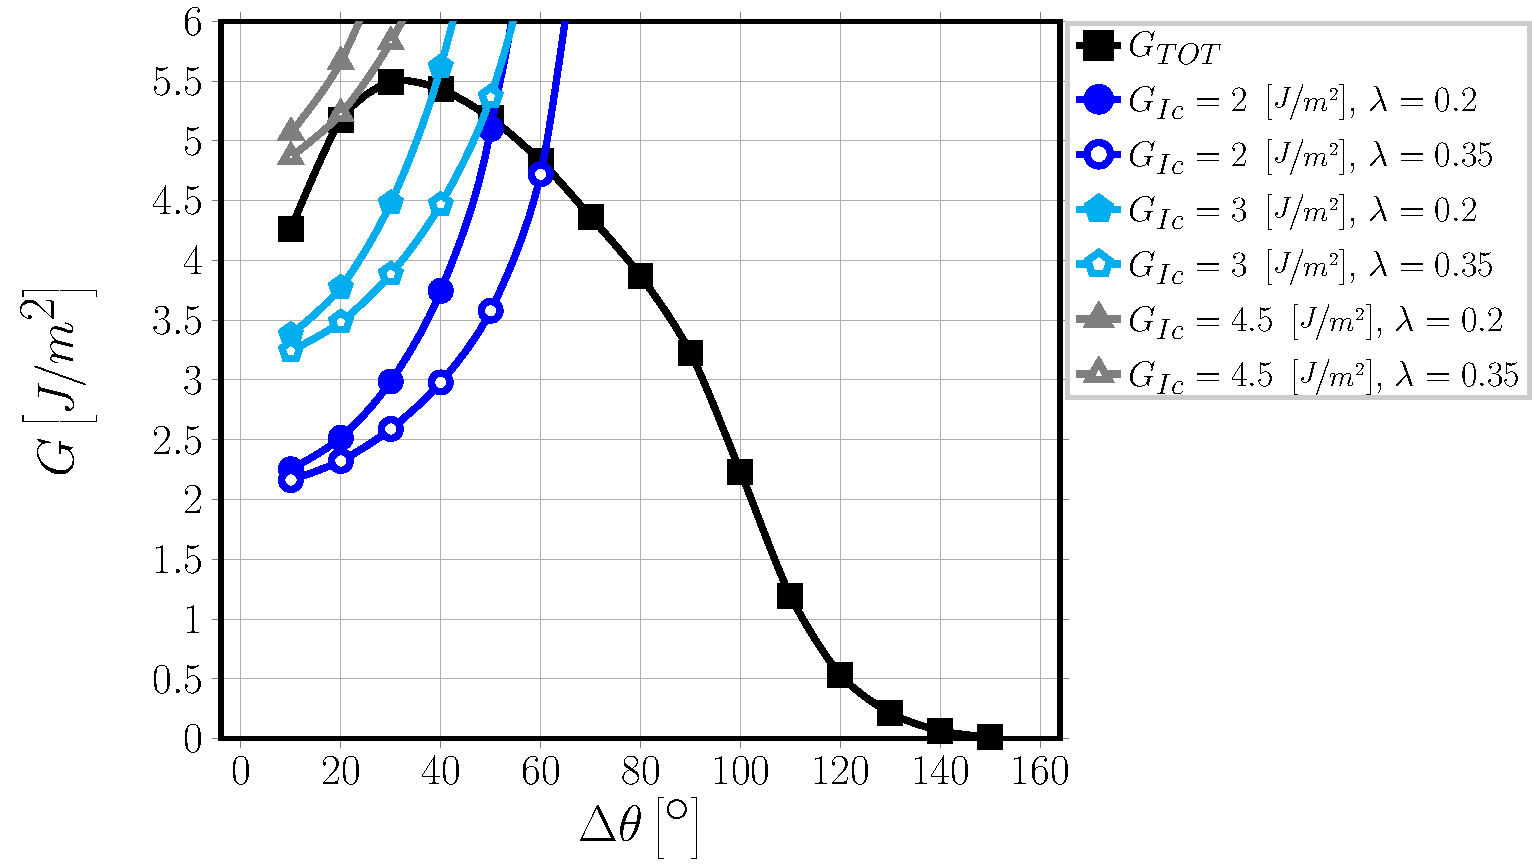
\includegraphics[width=0.45\textwidth]{vf60-dsize-S10A3.pdf}}\   
    \subfigure[$21\times 3-1\cdot t_{90^{\circ}}$]{\label{fig:debondsize-d}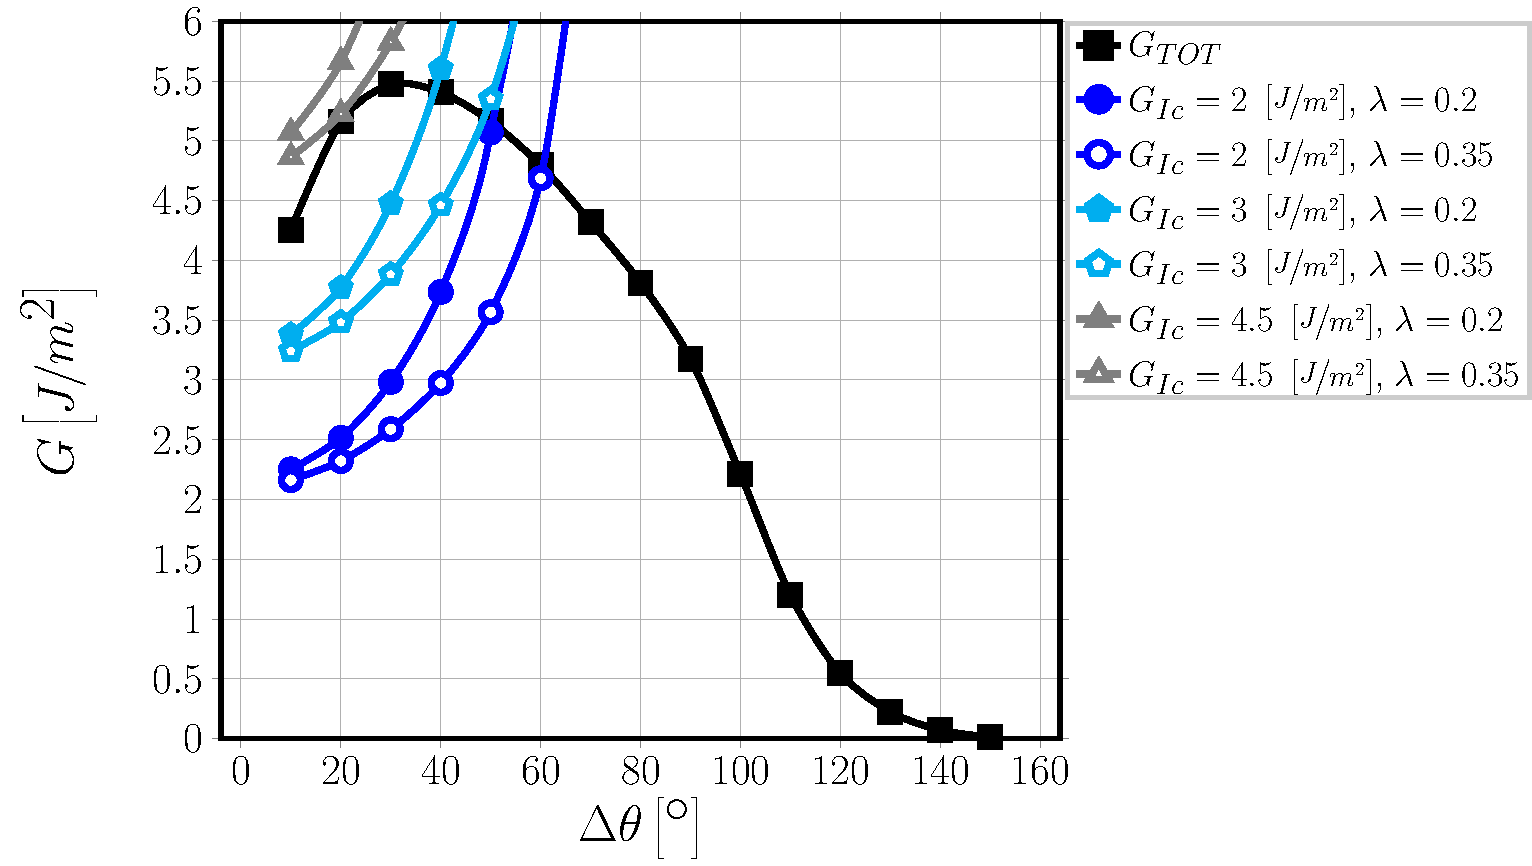
\includegraphics[width=0.45\textwidth]{vf60-dsize-S10A3T1.pdf}}\\
    \subfigure[$21\times 21-free$]{\label{fig:debondsize-e}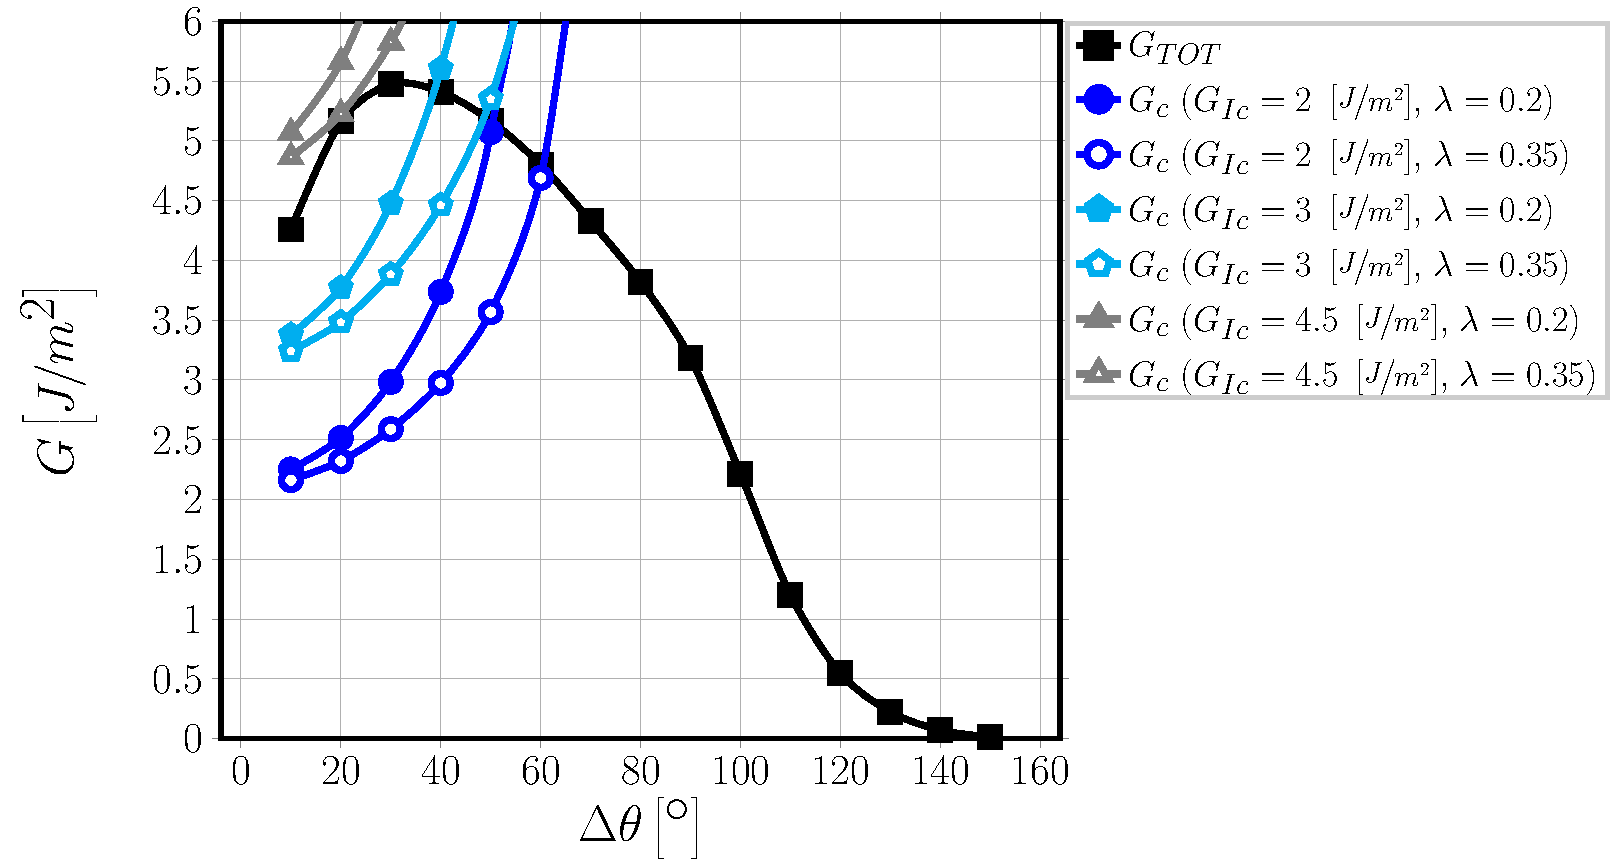
\includegraphics[width=0.45\textwidth]{vf60-dsize-S10A10.pdf}}\   
    \subfigure[$21\times 21-1\cdot t_{90^{\circ}}$]{\label{fig:debondsize-f}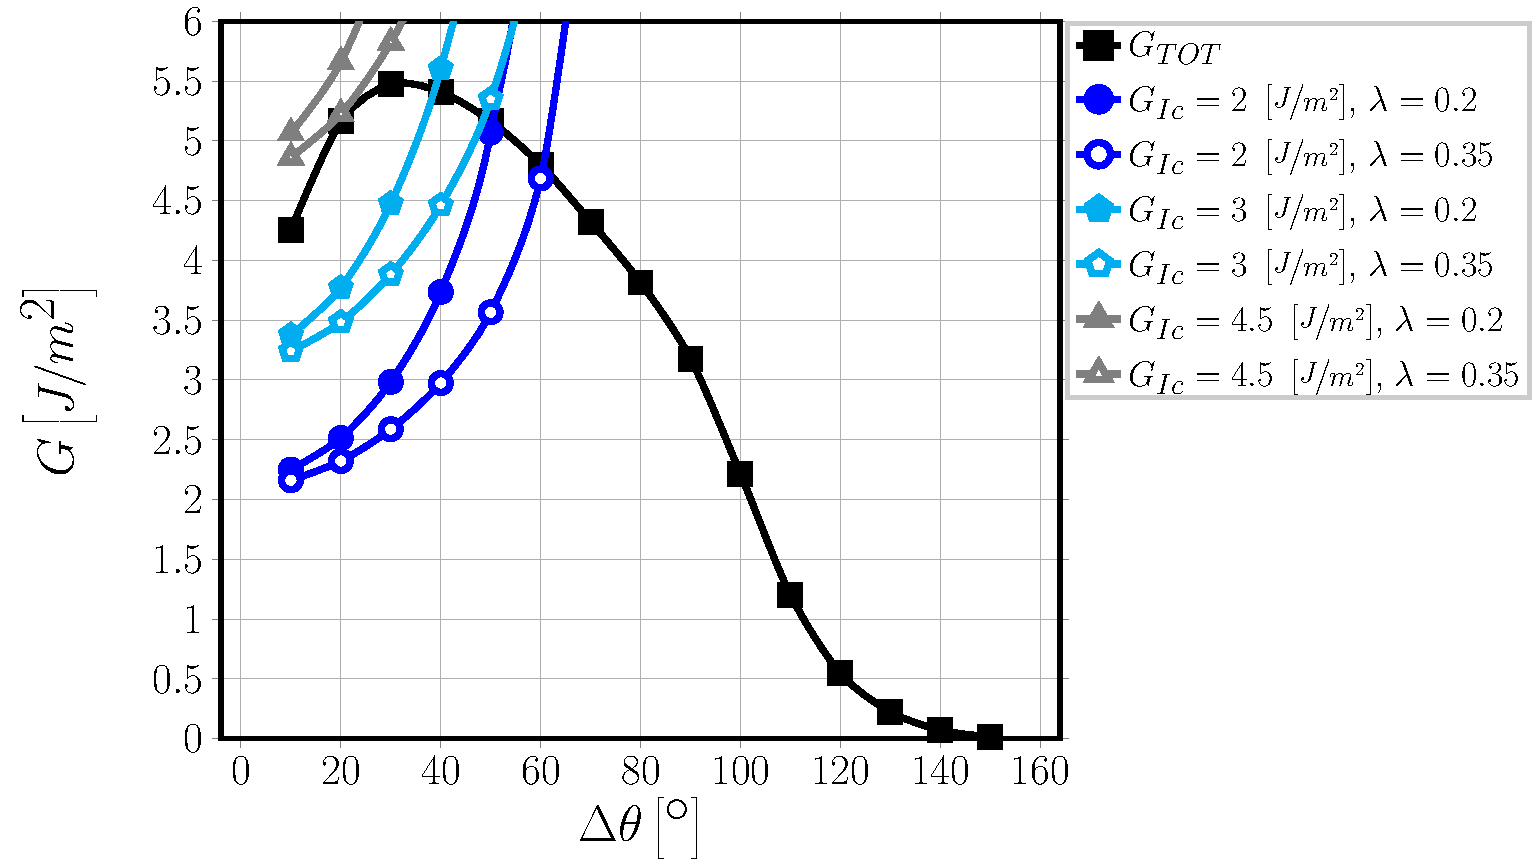
\includegraphics[width=0.45\textwidth]{vf60-dsize-S10A10T1.pdf}}\\
    \subfigure[$21\times 1-coupling$]{\label{fig:debondsize-g}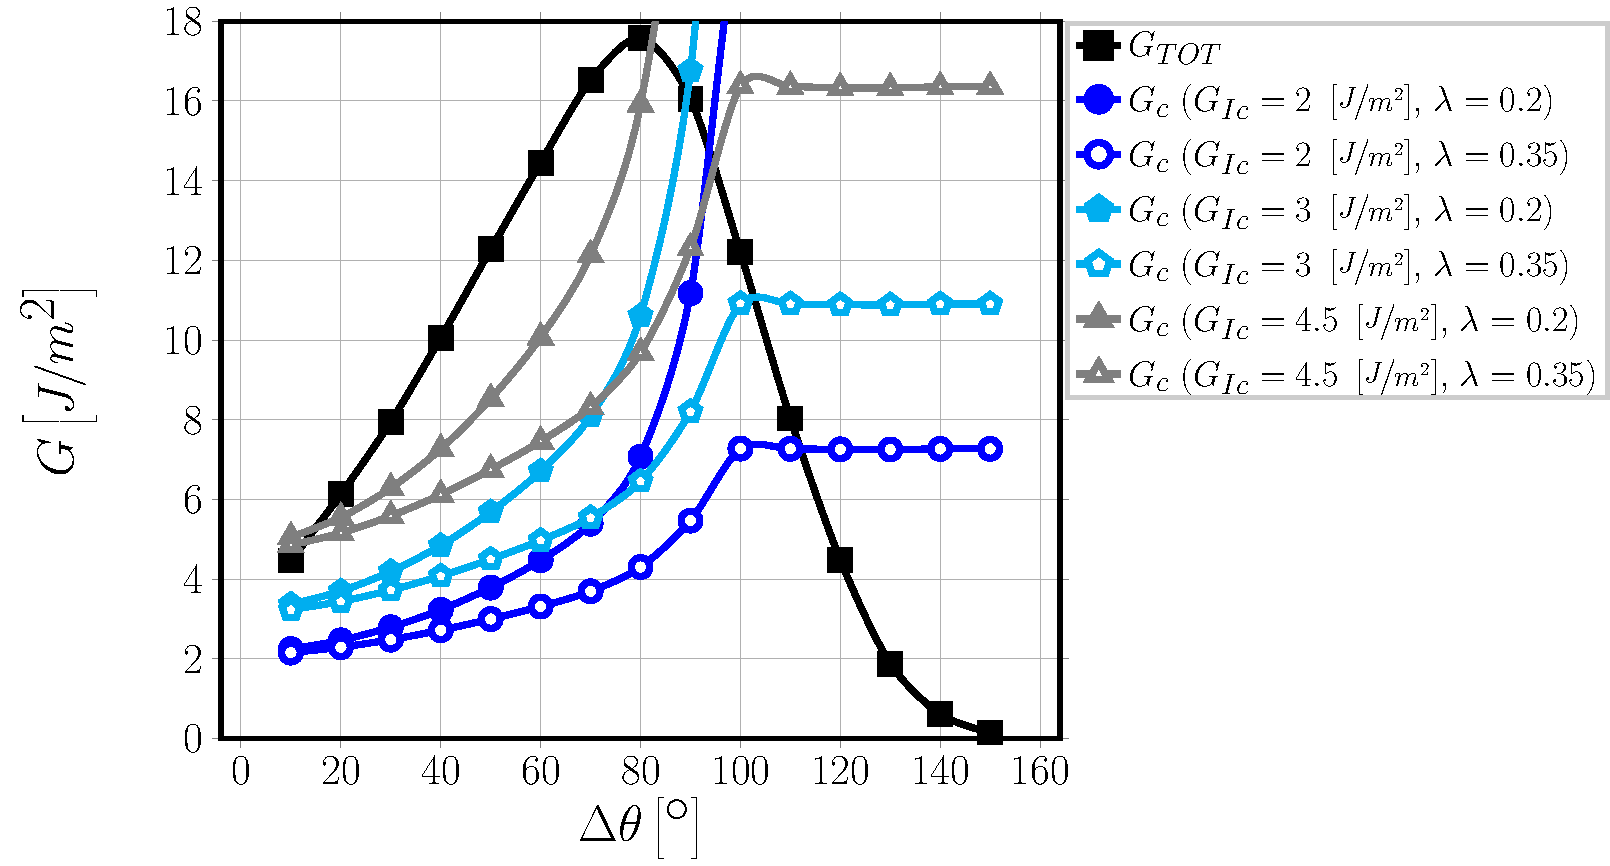
\includegraphics[width=0.45\textwidth]{vf60-dsize-S10A0vk.pdf}}\   
    \subfigure[$21\times 1-asymm$]{\label{fig:debondsize-h}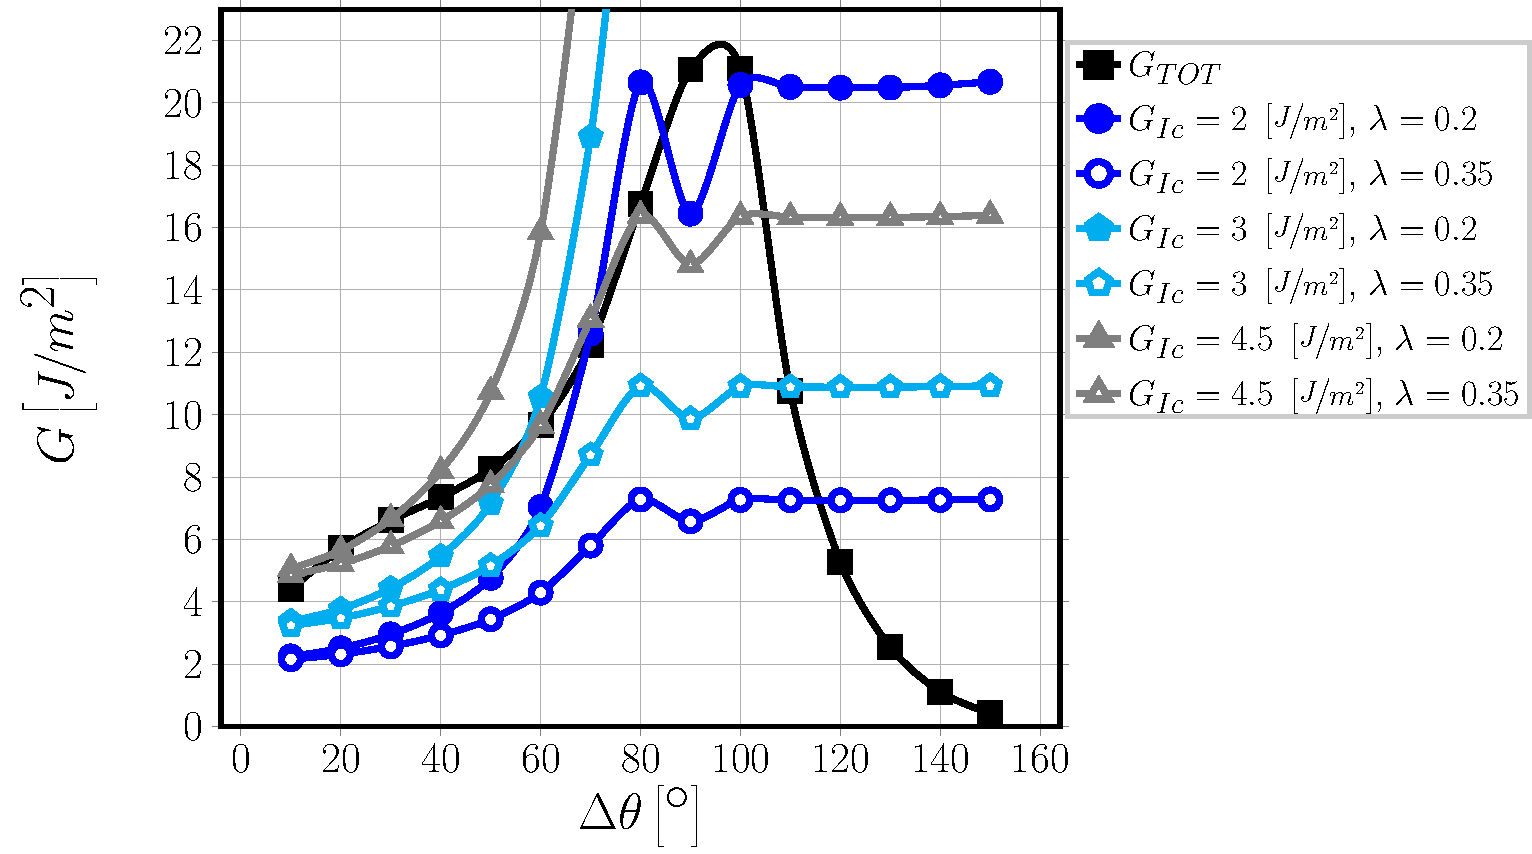
\includegraphics[width=0.45\textwidth]{vf60-dsize-S10A0asymm.pdf}}
\caption{Expected maximum size of debonds, for different RUCs and varying values of $G_{Ic}$ and $\lambda$.}\label{fig:debondsize}
\end{figure}

Comparison of Fig.~\ref{fig:debondsize-a} with Fig.~\ref{fig:debondsize-b} shows that the effect of the presence of the $0^{\circ}$ layer is to reduce the maximum size of debonds, from $\sim105^{\circ}$ in $21\times 1-free$ to $\sim45^{\circ}$ in $21\times 1-1\cdot t_{90^{\circ}}$ for $G_{Ic}=2\ \left[\frac{J}{m^{2}}\right]$, $\lambda=0.35$. However, the presence of just 1 ``row'' of undamaged fibers between the debond and the free surface or the $0^{\circ}/90^{\circ}$ interface (in RVEs respectively of UD composites and cross-ply laminates) makes the estimation of the maximum debond size unaffected by the number $k$ of fiber rows (Figures~\ref{fig:debondsize-c}, \ref{fig:debondsize-d}, \ref{fig:debondsize-e} and~\ref{fig:debondsize-f}). Moreover, for any given combination of $G_{Ic}$ and $\lambda$, the estimated debond size is the same for $n\times k-free$ and $n\times k-1\cdot t_{90^{\circ}}$ for $k\geq3$. The presence of a debond on the neighboring fiber in the vertical direction (RUCs $21\times 1-coupling$ and $21\times 1-asymm$) favors instead the growth of larger debonds (Figures~\ref{fig:debondsize-g} and~\ref{fig:debondsize-h}), with the largest size achieved when debonds are on opposite sides of consecutive fibers ($\sim115^{\circ}$ in $21\times 1-asymm$ and $\sim110^{\circ}$ in $21\times 1-coupling$). Considering the different combination of $G_{Ic}$ and $\lambda$, it is possible to identify the range of maximum debond propagation: for a 1-fiber row UD composite ($21\times 1-free$), $30^{\circ}-105^{\circ}$; for a 1-fiber row $90^{\circ}$ ply in a cross-ply laminate ($21\times 1-1\cdot t_{90^{\circ}}$), $30^{\circ}-45^{\circ}$; for a $k$-fiber row UD composite and a $k$-fiber row $90^{\circ}$ ply in a cross-ply laminate with $k\geq3$ ($21\times k-free$ and $21\times k-1\cdot t_{90^{\circ}}$), $40^{\circ}-60^{\circ}$; for consecutive debonds along the vertical direction in an infinite UD composite ($21\times 1-coupling$ and $21\times 1-asymm$), $80^{\circ}-110^{\circ}$ when debonds are on the same sides and $60^{\circ}-115^{\circ}$ when on opposite sides. These theoretical predictions are in striking agreement with the microscopical observations performed in~\cite{Correa2018} on $\left[0^{\circ}_{3},90^{\circ}_{3}\right]_{S}$ carbon fiber (AS4) - epoxy (8552) specimens subjected to tensile loading (corresponding to RUCs $n\times k-1\cdot t_{90^{\circ}}$ in this article). They report debond sizes in the range $21.4^{\circ}-89.2^{\circ}$ with average value of $49.3^{\circ}$ and standard deviation of $11.7^{\circ}$, with $63\%$ of the measurements in the range $40^{\circ}-60^{\circ}$.

\section{CONCLUSIONS}

Onset and propagation of fiber/matrix interface cracks has been studied in Representative Volume Elements (RVEs) of UD composites and $\left[0_{m\cdot k\cdot2L}^{\circ},90_{k\cdot2L}^{\circ},0_{m\cdot k\cdot2L}^{\circ}\right]$ laminates by means of Repeating Unit Cells (RUCs). Analysis of the stress distribution at the fiber/matrix interface in the absence of damage has shown that a stress criterion for initiation would predict, irrespectively of which criterion from those proposed in the literature is chosen, the onset of a debond at $0^{\circ}$ or $180^{\circ}$ with a semi-aperture $\Delta\theta_{0}$ in the range $2^{\circ}-12^{\circ}$, corresponding to a margin of $5\%$ on the satisfaction of the criterion. Assuming a mixed-mode criterion for debond propagation and taking into account the previous considerations regarding the stress distribution, the critical Mode I ERR $G_{Ic}$ is estimated to lie in the range $2-4.5\ \left[\frac{J}{m^{2}}\right]$. Estimation of maximum debond size finally provides: for a 1-fiber row UD composite, $30^{\circ}-105^{\circ}$; for a 1-fiber row $90^{\circ}$ ply in a cross-ply laminate, $30^{\circ}-45^{\circ}$; for a multiple fiber-rows UD composite and a multiple fiber-rows $90^{\circ}$ ply in a cross-ply laminate , $40^{\circ}-60^{\circ}$; for consecutive debonds along the vertical direction in an infinite UD composite, $80^{\circ}-110^{\circ}$ when debonds are on the same sides and $60^{\circ}-115^{\circ}$ when on opposite sides. These predictions agree well with the debond size distribution estimated in~\cite{Correa2018} through microscopic observations of cross-ply specimens.

\section*{ACKNOWLEDGEMENTS}

Luca Di Stasio gratefully acknowledges the support of the European School of Materials (EUSMAT) through the DocMASE Doctoral Programme and the European Commission through the Erasmus Mundus Programme.

\bibliographystyle{unsrt}

%\begin{thebibliography}{10}
%
%\bibitem{Barbero} E.J. Barbero, \textit{Finite Element Analysis of Composite Materials}. CRC Press, Boca Raton, 2008.
%\bibitem{Pimenta} S. Pimenta, S.T. Pinho, The effect of recycling on the mechanical response of carbon fibres and their composites. \textit{Composite Structures}, \textbf{94}, 3669-3684, 2012.
%
%\end{thebibliography}

\bibliography{refs}

\end{document}

